\documentclass[letterpaper]{article}

% \usepackage[letterpaper]{geometry}
\usepackage[log-declarations=false]{xparse}
\usepackage[quiet]{fontspec}
\usepackage{unicode-math}
\usepackage{amsmath}
\usepackage{amsthm}
\usepackage{amsfonts}
\usepackage{mathtools}
\usepackage{enumerate}
\usepackage{polyglossia}
\usepackage{graphicx}
\usepackage{tikz}
\usepackage{svg}

\setdefaultlanguage{spanish}

\newcommand{\vank}{\emph{Seifert-van Kampen} }

\theoremstyle{definition}
\newtheorem{definicion}{Definicion}

\theoremstyle{plain}
\newtheorem{teorema}{Teorema}

\theoremstyle{plain}
\newtheorem{corolario}{Corolario}

\theoremstyle{plain}
\newtheorem{lema}{Lema}

\theoremstyle{remark}
\newtheorem*{acotacion}{Acotacion}

\theoremstyle{remark}
\newtheorem{ejemplo}{Ejemplo}

\begin{document}
\title{Topologia algebraica}
\author{Ruben Astudillo \\ 201021009-k}
\date{\today}
\maketitle

\section{Prefacio}
Topología nos da un lenguaje para definir precisamente nociones como
compacidad, conjuntos cerrado e abierto y diferentes tipos de
separabilidad. Gran parte de estas propiedades tienen un carácter local,
es decir no son propiedades que definan al espacio total si no mas bien
por subparte de este. En el siglo XIX el mundo del álgebra, en
particular la teoría de grupos, había intentado y conseguido clasificar
progresivamente grupos de diferentes ordenes modulo isomorfismo. Habían
logrado esto a través de llamadas invariantes algebraicas, las cuales
eran preservadas a través de los isomorfismo de grupos. En topología se
deseaba hacer un tratamiento parecido para clasificar espacios, por lo
cual se necesitaba encontrar una invariante topológica. La elecciones de
esta no necesariamente nos dan teorías útiles, pues puede ser muy
general y no distinguir en propiedades que se consideran importantes. Si
hemos de tomar una propiedad como invariante topológica, sobre la cual
construir una teoría, esta no debe ser local. Idealmente nos gustaría
construir sobre alguna propiedad del espacio que fuera característica de
todo el espacio, algo en general notoriamente difícil. Resulta que si
nos reducimos a espacios arco-conexos podemos construir una respuesta
adecuada a través de los grupos fundamentales. Esta característica es
construida sobre clases de equivalencias de caminos cerrados, quienes
puedan deformarse entre si y permiten reificar información de los
``agujeros'' del espacio. Resulta que la elección de esta respuesta
tiene la consecuencia feliz de tener estructura de grupo subyacente, por
lo que nos permite reutilizar el trabajo ya realizado en el mundo del
álgebra para nuestro beneficio. Mas aun, las técnicas utilizadas en la
definición de este, son suficientemente abstractas como para ser
aplicado a otros dominios, lo cual motivo su estudio en propio interés
bajo el nombre de \emph{teoría de categorías}. Por lo que un
entendimiento de la topología algebraica es una buena introducción,
tanto practica como histórica, al lenguaje de categorías.

\tableofcontents
\section{Grupo fundamental}

{
\newcommand{\homRelAlt}{\stackrel{.}{\simeq}}
\subsection{Arcos y homotopías}
\begin{definicion}[Arco]
  Un arco en el espacio \(X\) es una función continua \(f : I \to X \)
  donde \(I = [0,1]\)
\end{definicion}
%% mariela: q1 ¿todo espacio 1-dimensional es homeomorfo a [0,1]?
%% no dije exactamente eso, un subconjunto convexo y acotado si lo es ,
%% pero debo de preguntar que se refiere
La definición tradicional es ligeramente mas general, cambiando que \(I\)
sea un subconjunto convexo acotado de un espacio unidimensional, pero
siempre podemos recuperar esta definición rescalando la distancia.

\begin{definicion}[Homotopía]
  Dados dos arcos \(f,g : I \to X\), diremos que \(f\) es homotópico a
  \(g\) si existe una función continua \(F : I \times I \to X \) tal que
  \[ \begin{matrix}
      F (x, 0) = f(x), & F (x, 1) = g(x)
     \end{matrix}
  \]
  Donde \(F\) sera llamada una homotopía entre \(f\) y \(g\). La
  existencia de dicha relación entre dos funciones sera denotada por \(f
  \homRelAlt g\).
\end{definicion}
\begin{figure}[h]
  \centering
  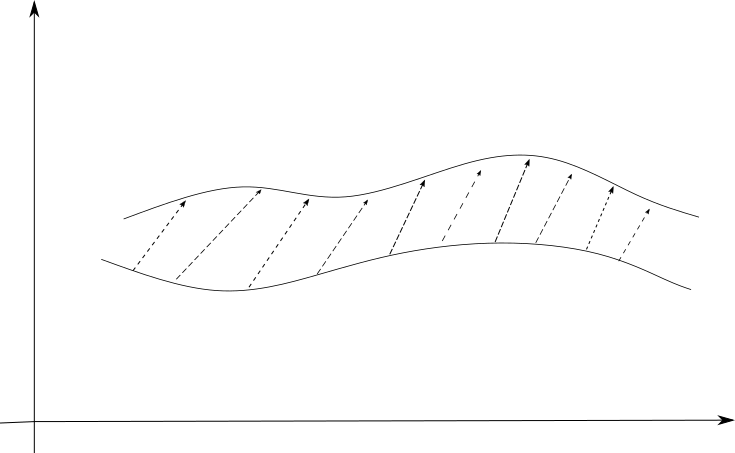
\includegraphics[scale=0.3]{./imagenes/homotopia.png}
  \caption{caracterización homotopía}
  \label{fig:homotopia-entre-funciones}
\end{figure}
Podemos pensar en el segundo argumento de una homotopía como el grado de
deformación entre dos funciones.
Si tratamos con arcos \(f,g : I \to X\) que posean los mismos puntos
iniciales y finales, es decir \(f(0) = g(0) = x_0, \; f(1) = g(1) =
x_1 \) podemos definir una relación homotópica ligeramente mas fuerte.

\begin{definicion}[Arco homotopía]
  \(f,g : I \to X\) son \emph{arco homotópicas} entre sí, si tienen los mismos
  puntos inicial y final \(x_0, x_1\) respectivamente y existe una homotopía entre
  ellos tal que cumpla
  \[
    \begin{matrix}
      F(s,0) = f(s), & F(s,1) = g(s) \\
      F(0,t) = x_0,  & F(1,t) = x_1
    \end{matrix}
  \]
  La existencia de esta relación entre dos funciones sera denotada por
  \(f \simeq g\).
\end{definicion}
% todo(slack) hacer algun dibujo de las homotopías entre las curvas
Una vez definida estas relaciones, una pregunta natural es si estas definen
una relación de equivalencia, ya que nos gustaría identificar clases de
curvas como elementos de alguna teoría algebraica. La respuesta es
afirmativa para ambas relaciones (el punto de inicio y final no juegan
un papel relevante). A continuación mostraremos que ``ser homotópicas''
es una relación de equivalencia.
\begin{teorema}
  \(\homRelAlt\) es una relación de equivalencia
\end{teorema}
\begin{proof}
  Hemos de probar que esta relación cumple la reflexividad, simetría y
  transitividad. Sean \(f,g,h : I \to X\) tres arcos arbitrarios.
  \begin{itemize}
  \item La reflexividad es directa pues la función \(F(x,t) = f(x)\) es
    una deformación continua de \(f\) a \(f\), por tanto \(f \homRelAlt
    f\).

  \item La simetría se obtiene de invertir el sentido de deformación de la
    homotopía original. Formalmente, dado \(f \stackrel{.}{\simeq} g\)
    tenemos una homotopía entre estas \((x,t) \mapsto F(x,t)\). A partir
    de aquí podemos definir
    \begin{equation}
      \label{eq:homotopy-simetry}
      (x,t) \mapsto \hat{F}(x,t) := F(x,1-t)
    \end{equation}
    con \(\hat{F}\) una homotopía entre \(g\) y \(f\). Por tanto \(g
    \stackrel{.}{\simeq} f\).

  \item La transitividad se obtiene a partir de de dividir \(I\) en dos
    intervalos donde se deformen individualmente cada homotopía al doble
    del grado. Formalmente dado \(f \stackrel{.}{\simeq} g\) y \(g
    \stackrel{.}{\simeq} h\) representadas por las homotopías \(F\) y
    \(G\) respectivamente, se define
    \[ FG(x,t) = \begin{cases}
        F(x,2t) & t \in [0,\frac{1}{2}] \\
        G(x,2t - 1) & t \in [ \frac{1}{2} , 1]
      \end{cases}
    \]
    Esta es una deformación continua claramente en \((x,t) \in I \times
    [0, \frac{1}{2}) \cup I \times (\frac{1}{2}, 1]\). La continuidad en
    \(I \times \{\frac{1}{2}\}\) proviene de la consistencia en dicho
    punto de ambas homotopías
    \[ F(x,2 \cdot \frac{1}{2}) = g(x) = G(x, 2 \cdot \frac{1}{2} - 1)\]
    lo que nos permite utilizar el \emph{lema del pegamiento}
    \cite[p.~108]{munkres} para obtener la continuidad de \(FG\).
    Obteniendo así \(f \stackrel{.}{\simeq} h\).
  \end{itemize}
\end{proof}

En análisis real, es común trabajar con conjuntos convexos. En arcos
sobre estos conjuntos, veremos una homotopía repetidamente llamada
homotopía de linea recta.
\begin{definicion}[Homotopía de linea recta]\label{def:homotopia-linea}
  Sean \(f,g : I \to X\) dos arcos arbitrarios y sea \(\mathcal C
  \subset X\) un subconjunto convexo. Si \(f(I),g(I) \subset \mathcal
  C\), entonces se define la homotopía de linea recta por
  \[ F(x,t) := (1-t) \cdot f(x) + t \cdot g(x) \]
\end{definicion}
\begin{acotacion}
  En la definición anterior, la continuidad de \(F\) se obtiene de ser
  una combinación convexa de funciones continuas \(f\) y \(g\). De que
  sea una combinación convexa se obtiene la importancia de que existe un
  conjunto \(\mathcal C \subset X\) que contenga a las imágenes.
\end{acotacion}

Con estas definiciones ya podemos empezar a hablar de \([f]\) clases
de equivalencia de funciones bajo una relación homotópica
\[ [f] = \{ g : I \to X \mid f \stackrel{.}{\simeq} g \} \]
Notar que la construcción es valida para las dos relaciones aunque por
nuestra meta de construir el grupo fundamental nos interesa
principalmente la relación arco homotópica, por razones a estudiar mas
adelante.

\subsection{Grupoide de arcos}
Si tenemos dos arcos continuos \(f,g\) tales que el punto final de \(f\)
sea el punto inicial de \(g\) podemos construir un camino continuo que
recorra \(f\) luego recorriendo \(g\). Esta idea es conocida formalmente
como el producto de dos arcos.

\begin{definicion}[Producto de arcos]
Para dos arcos \(f,g : I \to X\) tales que
\(f(1) = g(0)\), se define el producto \(f * g \)
\[ (f*g) (s) \coloneqq \begin{cases}
    f(2s) & s \in [0,\frac{1}{2}] \\
    g(2s - 1) & s \in [\frac{1}{2} , 1]
  \end{cases}
\]
la cual sigue siendo una funcion continua en virtud del lema del
pegamiento.
\end{definicion}

Esta construccion se puede reutilizar para clases
\emph{arco}-homotopicas \([f],[g]\) que compartan punto final e inicial
respectivamente para definir un producto de clases de equivalencia
\[ [f] * [g] \coloneqq [f * g]\]
El cual esta bien definido pues si \(f \simeq f' ,\ g \simeq
g'\) a traves de las homotopias \(F, G\) respectivamente, entonces
\[
  H(s,t) = \begin{cases}
    F(2s,t) & s \in [0, \frac{1}{2}] \\
    G(2s - 1, t) & s \in [\frac{1}{2} , 1]
  \end{cases}
\]
Es la homotopia que relaciona a los arcos que sean homotopicos a
\(f*g\). Esta ademas es continua en virtud otra vez del lema del pegamiento.

\paragraph{} Con esta operacion binaria, una pregunta a hacerse es si
\((\mathcal C (I , X)/\simeq , (*))\) tiene posee estructura de
grupoide, esto equivale a cumplir 3 propiedades
\begin{enumerate}
\item \textbf{Asociatividad} Si \([f] * ([g] * [h])\) esta definido entonces
  tambien lo debe estar \(([f] * [g]) * [h]\) y ademas deben coincidir.
\item \textbf{Identidades izquierda y derecha} Para todo \([f]\) con
  \(x_0, x_1\) puntos inicial y final respectivamente, debe de
existir elementos \([k_{x_0}], [k_{x_1}]\) tales que
\[ \begin{matrix}
    [f] * [k_{x_1}] = [f] & & [k_{x_0}] * [f] = [f]
  \end{matrix}
\]
\item \textbf{Inverso} Para todo \([f]\) clase de arcos con \(x_0, x_1\)
  puntos inicial y final respectivamente debe de existir un elemento
  \([f^{-1}]\) que cumpla
\[ \begin{matrix}
    [f] * [f^{-1}] = [k_{x_0}] & & [f^{-1}] * [f] = [k_{x_1}]
  \end{matrix}
\]
\end{enumerate}
Para probar esto necesitamos primero definir a nuestros candidatos de
\(k_{x_0}, k_{x_1}, f^{-1}\) ademas de algunas funciones auxiliares,
iniciando por los mapeos constantes e identidad en \(I \to I\)
\[ \begin{matrix}
     e_0 : & I \to I & e_0(t) \coloneqq 0 \\
     e_1 : & I \to I & e_1(t) \coloneqq 1 \\
     i :   & I \to I & i(t) \coloneqq t \\
     \bar{i} : & I \to I & i(t) \coloneqq 1 - t
   \end{matrix}
   \]
Ademas, para todo arco \(f : I \to X \), el elemento \(f^{-1} : I \to X \) esta
definido (en el espiritu de \eqref{eq:homotopy-simetry}) por
\[ f^{-1} (s) \coloneqq f (1 - s) \]
Por ultimo, para todo \(x \in X \) se define la curva
constante\footnote{\(k\) por \emph{konst}}
\begin{align*}
  k_x : &I \to X \\
        &t \mapsto x
\end{align*}
Con esto podemos afrontar la demostración
\begin{proof}
Se procedera en orden \(2 \to 3 \to 1\) con lemas en medio. Sea \(f : I
\to X\) el representante de la clase \([f]\). sean \(x_0, x_1\) los
puntos inicial y final de \(f\) respectivamente.

\paragraph{(2).} Dados \(i,e_1\) arcos en \(I\) definidos anteriormente,
es claro que \(i * e_1\) es tambien un arco (continuo) en \(I\); mas aun,
ya que \(I = [0,1]\) es convexo, se tiene \(i * e_1 \simeq i\) con la
homotopia de la linea recta entre estos denotada por \(C\).

Tambien conocemos que la composición de funciones continuas es
continua, de lo cual podemos decir que dada una homotopia \(H : I \times
I \to I\) la composicion \( f \circ H : I \times I \to X\) es una homotopia.

Por otro lado, necesitamos conocer como se comporta la composicion con
respecto a nuestro producto \((*)\), para esto tenemos el siguiente lema
\begin{lema}[Distributividad de la composicion sobre producto]
\label{lema:dist-composicion-producto}
\[\forall a,b : I \to I,\ \forall f : I \to X,\ f \circ (a * b) = (f
\circ a) * (f \circ b) \]
\end{lema}
\begin{proof}
  \[ f \circ (a*b) (s) =
    \begin{cases}
      f (a(2s)) & s \in [0,\frac{1}{2}] \\
      f (b(2s - 1)) & s \in [\frac{1}{2} , 1]
    \end{cases}
    = (f \circ a) * (f \circ b) (s)
  \]
\end{proof}

Luego esto nos permite afirmar en especifico que
\[ f \circ i \simeq f \circ (i * e_1) = (f \circ i) * (f \circ e_1) \]
en virtud de la homotopia
\[ f \circ C : I \times I \to X \]
Por tanto
\begin{equation}\label{eq:homequiv2.1}
[f \circ i] = [f \circ (i * e_1)] = [(f \circ i) * (f \circ e_1)]
\end{equation}
Si tomamos este ultimo termino, sabemos que por definicion
\begin{equation}\label{eq:homequiv2.2}
[(f \circ i) * (f \circ e_1)] = [(f \circ i)] * [(f \circ e_1)]
\end{equation}
y es claro tambien que
\[
  \begin{matrix}
    f \circ i = f & f \circ e_1 = k_{x_1} \\
  \end{matrix}
\]
\begin{equation}\label{eq:homequiv2.3}
[(f \circ i)] * [(f \circ e_1)] = [f] * [k_{x_1}]
\end{equation}
juntando
\eqref{eq:homequiv2.1},\eqref{eq:homequiv2.2},\eqref{eq:homequiv2.3} nos
muestra que \([k_{x_1}]\) es la identidad por la derecha. Podemos
hacer un proceso analogo para \([k_{x_0}]\) como identidad por la
izquierda, asi probando (2).

\paragraph{(3).} De manera similar a la pregunta anterior, notar que \(i,
\bar{i}\) definidos anteriormente cumplen
\[ i * \bar{i} \simeq e_0 \]
por la homotopia de linea recta en el espacio \(I\) que es convexo.
Utilizando el lemma \eqref{lema:dist-composicion-producto} tenemos que
\[ [f * f^{-1}] = [f \circ (i * \bar{i})] = [f \circ e_0] = [k_{x_0}] \]
\[ \implies [f] * [f^{-1}] = [k_{x_0}] \]
De manera analoga se prueba la inversa por la izquierda.

\paragraph{(1).}
Por definicion, tenemos que las diferentes asociaciones nos resultan en
diferentes representates de clase
\[
  \begin{matrix}
    (f * g) * h \, (t) =
    \begin{cases}
      f (4t), & t \in [0, \frac 1 4] \\
      g (4t - 1), & t \in [\frac 1 4, \frac 1 2] \\
      h (2t - 1), & t \in [\frac 1 2, 1] \\
    \end{cases} &
    f * (g * h) \, (t) =
    \begin{cases}
      f (2t), & t \in [0, \frac 1 2] \\
      g (4t - 2), & t \in [\frac 1 2, \frac 3 4] \\
      h (4t - 3), & t \in [\frac 3 4, 1] \\
    \end{cases}
  \end{matrix}
\]
Sea \(T : I \to I\) definida por
\[ T (t) :=
  \begin{cases}
    2t & t \in [1 , \frac 1 4] \\
    t + \frac 1 4 & t \in [\frac 1 4, \frac 1 2] \\
    \frac t 2 + \frac 1 2 & t \in [\frac 1 2, 1]
  \end{cases}
\]
\(T\) es una funcion continua por el lema del pegamiento. Por ser \(I\)
un dominio convexo, se tiene que \(i \simeq T\), luego
\[ [(f * g) * h] = [\big( (f * g) * h \big) \circ i] = [\big( (f * g) *
  h \big) \circ T ] = [f * (g * h)] \]
\end{proof}


\subsection{Grupo fundamental}
Sobre nuestros arcos tenemos una estructura de grupoide porque no siempre
podemos hacer coincidir los puntos inicial y final. Si nos fijáramos en
un solo punto \(x_0 \in X\) tal que todas los arcos \(f : I \to X\)
cumplieran que
\[ f(0) = x_0 = f (1) \]
Entonces las propiedades que demostramos anteriormente nos dirían que el
espacio \((X / \simeq, *)\) es un grupo algebraico.
\begin{definicion}[Grupo fundamental]
  Sea \(X\) un espacio topológico y \(x_0 \in X\) un punto. La colección
  \[ \pi_1 (X,x_0) = \{ [f] \mid f : I \to X, f \text{ continua}\}\]
  \[ [f] := \{ g : I \to X \mid f \simeq g\}\]
  junto con el producto de caminos \((*)\) forman el llamado
  \textbf{grupo fundamental} \((\pi_1(X,x_0), (*))\)
\end{definicion}

Nuestro interés es mostrar que para un espacio dado, su grupo
fundamental es una invariante topológica. Esto quiere decir que dado dos
espacios puntuados \((X,x_0)\) e \((Y,y_0)\) homeomorfos, debe de
existir un respectivo isomorfismo de grupos entre \(\pi_1(X,x_0)\) y
\(\pi_1(Y,y_0)\). Para esto debemos recordar que un isomorfo entre
grupos es un homomorfismo, inyectivo y sobreyectivo.
\begin{definicion}
  Sean \((G,(*)), (G', (\cdot))\) dos grupos algebraicos. \(F : G \to
  G'\) es un homomorfismo entre grupos si y solo si
  \[ \forall x,y \in G,\ F (x * y) = F(x) \cdot F(y)\]
\end{definicion}
% Mariela me dijo que esto es un corolario, no se si si quiera es
% necesario.
\begin{corolario}
  \[ e \text{ es identidad de } G \implies F(e) \text { es identidad de } G' \]
\end{corolario}

\subsubsection{Ejemplo intuitivo de \(\mathbb{R}^2 - \{(1,1)\}\).}
Para mostrar la intuición detrás de la definición, utilizaremos como
ejemplo un espacio relativamente sencillo de visualizar. hemos de
caracterizar todas la curvas cerradas que inicien en un punto
arbitrario, que denotaremos por \(x_0\). Sea \(f : I \to \mathbb{R}^2 -
\{(1,1)\}\) un camino arbitrario, con dicho punto inicial, tendremos
tres grandes alternativas para de su clasificación.
\begin{figure}[h]
  \centering
  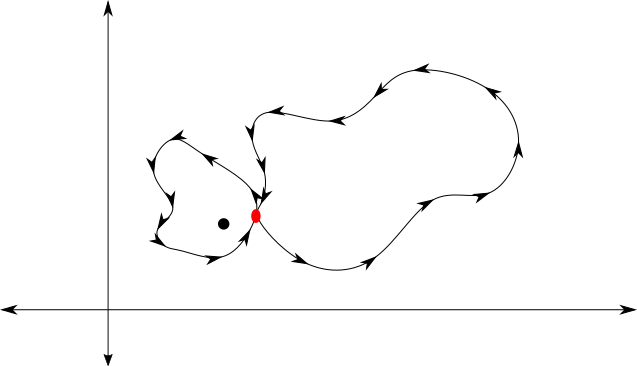
\includegraphics[scale=0.5]{./imagenes/R2-punto.png}
  \caption{\(R^2\) sin el punto \((1,1)\) en negro. Origen en rojo. }
  \label{fig:R2-sin-punto}
\end{figure}
\begin{itemize}
\item La curva denotada por \(f\) puede estar contenida en un subconjunto
  convexo de \(R^2 - \{(1,1)\}\). De esta manera, la curva pertenece a la
  homotopía de la linea recta dada por la definicion
  \ref{def:homotopia-linea} bajo la función
  \[ L (t,\lambda) = \lambda f (t) - (1 - \lambda) k_{x_0} (t)\]
  Por lo tanto en este caso, \(f \in [k_{x_0}]\).
\item La curva \(f\) no puede ser contenida en un subconjunto convexo de
  \(R^2 - \{ (1,1)\}\). Esto solo puede suceder si la curva \(f\)
  encerrara al punto \(x_0\), de manera que la relación \(\lambda x +
  (1 - \lambda) y\) no seria valida para algunos \(\lambda, x, y\). Por
  tanto \(f \not \in [k_{x_0}]\), así que denotaremos a la clase de
  equivalencia a la que pertenezca como \([\mathtt{F}^1]\).
\item La curva \(f\) encierra a \(x_0\) \(2\) veces. Podemos definir dos
  caminos \(g_1, g_2\) tales que \(f = g_1 * g_2\) (modulo re-escalamiento
  en parámetros) y que \(g_1, g_2 \in \mathtt F ^1\). Esto no diría que
  \( f \in [\mathtt F ^1] * [\mathtt F ^1] =: [\mathtt F ^2]\). Este
  procedimiento puede generalizar para todos los naturales.
% \item La curva \(f\) encierra a \(x_0\) \(2\) veces. Dado que cada vez
%   que lo encierra, esa curva (hasta ese momento) es homotopica a
%   \([\mathtt F ^1]\), tenemos que \(f\) es isometrica a \( [\mathtt F
%   ^1] * [\mathtt F ^1] =: [\mathtt F ^2]\). Esto se puede generalizar
%   para todos los naturales.
\end{itemize}
Así intuitivamente vemos que para este tenemos las clase de
equivalencias \([k_{x_0}], [\mathtt F ^1], [\mathtt F ^2], \dots \) con
la propiedades algebraicas
\[ [k_{x_0}] * [\mathtt F ^n] = [\mathtt F ^n] * [k_{x_0}]\]
\[ [\mathtt F ^m]  * [\mathtt F ^n] = [\mathtt F ^{n + m}]\]
En efecto, estos elementos son bajo isomorfismo de grupo equivalentes a
el grupo \((\mathbb{Z}, +)\). Por tanto diremos que este es el grupo
fundamental de \(R^2 - \{(1,1)\}\).

\paragraph{} Cabe notar que esta no es una demostración formal, no se ha demostrado
que estas son todas alternativas posibles de curvas, de lo cual depende
todo nuestro argumento. Mas adelante daremos una demostración formal de
que esta intuición es la correcta, pero por ahora sirve como marco
conceptual del objeto que estamos estudiando.

\subsection{Importancia punto de origen}
En el ejemplo anterior se vio que el punto \(x_0\) la verdad no
jugaba ningún papel importante, su única misión era identificar el
origen de los caminos. En espacios como el anterior, la importancia de
la elección se ve reducida puesto que este es arco-conexo, en estos
espacio \(\forall a,b \in X\), con \(X\) un espacio topológico a
estudiar, existe un camino \(\alpha : I \to X\) tal que \(\alpha (0) =
a,\ \alpha (1) = b\). Si nuestro espacio \(X\) no fuera arco-conexo,
caemos en la disyuntiva de elegir un punto apropiado que represente
``suficientemente'' al espacio, en la definicion de su grupo.
fundamental. Dada que la motivacion de definir en primer lugar el grupo
fundamental provenia de establecer una \emph{invariante} topologica,
hace dudar que la parametrizacion en cuanto a punto base del grupo
fundamental indique que procedemos por buen camino
%todo(slack): buscar papers de grupo fundamental de conjuntos conexos y
%no arco conexos

Aun en espacios arco-conexos seguimos declarando el punto base con
respecto al cual derivamos su grupo fundamental. Para ver con mas
claridad el por que, primero debemos probar que en efecto, en espacios
arco-conexos el grupo fundamental no depende del punto de partida.
\begin{teorema} \label{not:alpha-hat}
  Sea \(x_0 , x_1 \in X\) puntos de un espacio arco conexo, sean \(\pi
  (X, x_0), \pi (X, x_1)\) dos grupos fundamentales de \(X\)
  parametrizados por estos puntos, entonces estos dos grupos son isomorfos
\end{teorema}
\begin{proof}
  Por ser \(X\) arco-conexo, existe \(\alpha : I \to X\) camino
  continuo, tal que \(\alpha (0) = x_0,\ \alpha (1) = x_1\). Se define
  la funcion
  \begin{align*}
    \hat \alpha : \pi (X, x_0) &\to \pi (X, x_1) \\
    [g] &\mapsto [ \alpha^{-1} * g * \alpha ]
  \end{align*}
  Esta funcion, esta bien definida puesto que \(\forall g \in \pi (X,
  x_0),\ \alpha^{-1} * g * \alpha \) es continua (en virtud de \(*\)).
  Sea entonces por definicion y reduccion se tiene
  \[ \alpha^{-1} (t) = \alpha (1 - t)\]
  \[\big(\alpha^{-1} * g * \alpha \big) (0) = \alpha (1 - 0) = x_1 = \alpha (1) =
    \big(\alpha^{-1} * g * \alpha \big) (1)\]

  \paragraph{\(\hat \alpha\) es homomorfismo.} Para esto, se procede por
  definicion. Por un lado, al mapear la identidad de \(k_{x_0} \in \pi
  (X, x_0) \), tenemos por reduccion
  \begin{align*}
    \hat \alpha ([k_{x_0}])
                 &= [\alpha^{-1} * k_{x_0} * \alpha] \\
                 &= [\alpha^{-1}] * [k_{x_0} * \alpha] \\
                 &= [\alpha^{-1}] * [\alpha] \\
                 &= [\alpha^{-1} * \alpha] \\
                 &= [k_{x_1}] \\
  \end{align*}
  Por otro lado, si \(u,v \in \pi (X, x_0) \), tenemos la siguiente
  reduccion del producto
  \begin{align*}
    \hat \alpha ([u] * [v]) &= [\alpha^{-1} * u * v * \alpha] \\
    &= [\alpha^{-1} * u * k_{x_0} * v * \alpha] \\
    &= [\alpha^{-1} * u * \alpha * \alpha^{-1} * v * \alpha] \\
    &= [\alpha^{-1} * u * \alpha ] * [ \alpha^{-1} * v * \alpha] \\
    &= \hat \alpha (u) * \hat \alpha (v) \\
  \end{align*}

  \paragraph{\(\hat \alpha\) es inyectiva y sobreyectiva.} La inyectividad es
  clara, pues si \([u],[v] \in \pi (X, x_0),\ [u] \not \simeq [v]
  \implies [\alpha^{1}] * [u] * [\alpha] \not \simeq [\alpha^{-1}] * [v]
  * [\alpha]\). Para ver la sobreyectividad, notemos que \(\forall [k] \in
  \pi (X, x_1) \), siempre existe \( [\alpha * k * \alpha^{-1}]\) tal
  que
  \[ \hat \alpha ([\alpha * k * \alpha^{-1}]) = [\alpha^{-1} * \alpha * k *
    \alpha^{-1} * \alpha] = [k]\]
  Por tanto \(\hat \alpha\) es un isomorfismo de grupos.
\end{proof}
En el la prueba anterior, la existencia del camino \(\alpha\)
parametrizaba que tipo de isomorfismo \(F\) que construiamos, es decir
nuestro \(F\) enrealidad era \(F_{\alpha}\). La eleccion de punto bases
\(x_0, x_1\), nos permite hablar de la existencia de unico o multiples
isomorfimos entre grupos fundamentales \(\pi (X, x_0), \pi (X, x_1) \),
dependientes de la cantidad de caminos entre \(x_0\) y \(x_1\) que
existan. Esto es un tema importante a considerar, puesto que existe un
caracterizacion de \(\pi (X, x_0) \) como grupo abeliano, que depende de
la cantidad de estos isomorfismos.
\begin{teorema}
  Sean \(x_0, x_1 \in X\) puntos en un espacio arco-conexo. El grupo
  \(\pi (X, x_0) \) es abeliano si y solo si \(\forall \alpha, \beta\)
  caminos (distintos) entre \(x_0\) y \(x_1\), se cumple que \(F_\alpha =
  F_\beta\), con \(F_{\xi} ([f]) = [\xi^{-1} * f * \xi] \)
\end{teorema}
\begin{proof}
  Procedemos por la implicacion original. Dado que \(\pi (X, x_0)\) es
  abeliano, esto significa que \(\forall [f],[g] \in \pi (X, x_0),\ [f]
  * [g] = [g] * [f]\). Sean \(\alpha, \beta\) caminos entre \(x_0,x_1\)
  fijos pero arbitrarios, para mostrar que \(F_\alpha = F_\beta\),
  debemos mostrar que para todo argumento, los resultados coinciden. Sea
  \([f] \in \pi (X, x_0) \) un argumento fijo pero arbitrario. Dado que
  \(\alpha * \beta^{-1} * \beta \simeq \alpha \), se tiene que
  \(F_\alpha = F _{\alpha * \beta^{-1} * \beta}\), luego por definicion
  se cumplen la siguientes reducciones
  \[ F_\alpha ([f]) = F_{\alpha * \beta^{-1} * \beta} ([f]) =
    [\beta^{-1}] * [\beta * \alpha^{-1}] * [f] * [\alpha * \beta^{-1}]
    * [\beta] \]
  Donde \(\alpha * \beta^{-1} \in \pi (X, x_0) \), por lo tanto podemos
  aplicar conmutatividad con \([f] \in \pi (X,x_0)\) obteniendo la expresion
  \[ [\beta^{-1}] * [\beta * \alpha^{-1}] * [\alpha * \beta^{-1}] * [f]
    * [\beta] = [\beta^{-1}] * [f] * [\beta] = F_\beta ([f]) \]
  probando asi lo buscado.

  En el converso, sean \([f],[g] \in \pi (X, x_0) \) fijos pero
  arbitrarios, dado que \(\alpha\) es camino entre \(x_0\) e \(x_1\), se
  tiene que \(f * \alpha\) tambien es camino entre \(x_0\) e \(x_1\).
Por hipotesis, tenemos en particular para estos caminos, que se cumple
la relacion
  \begin{align*}
    F_{f * \alpha} ([g]) &= F_{\alpha} ([g]) \\
    [(f * \alpha)^{-1} * g * (f * \alpha) ] &= [\alpha^{-1} * g * \alpha] \\
    [\alpha^{-1} * f^{-1} * g * f * \alpha ] &= [\alpha^{-1} * g * \alpha] \\
    [\alpha^{-1}] * [f^{-1}] * [g] * [f] * [\alpha] &= [\alpha^{-1}] *
        [g] * [\alpha] \\
    [f^{-1}] * [g] * [f] &= [g] \\
    [g] * [f] &= [f] * [g], \qquad \forall [f],[g] \in \pi (X, x_0) \\
  \end{align*}
\end{proof}
En resumen si sabemos que \(\pi (X, x_0)\) es abeliano, esto equivale a
decir que \(\forall \alpha,\beta\) caminos entre \(x_0, x_1\), se tiene
que existe un \emph{unico} isomorfismo entre \(\pi (X,x_0) \) y \( \pi
(X,x_1)\), pues \(F_\alpha = F_\beta\). Anteriormente, teniamos la
existencia de posiblemente multiples isomorfismos entre \(\pi (X, x_0)
\) y \(\pi (X, x_1) \). Si no podemos parametrizar los isomorfismos
entre distintos puntos bases de un grupo fundamental, perdemos esta
caractizacion de grupo fundamental abeliano, pues perdemos la capacidad
de contar cuantos isomorfismos existen.

\subsection{Invariante topologica}
Nuestra meta original era mostrar que los grupos fundamentales son una
invariante topologica de un espacio, es decir, dados \(X,Y\) dos
espacios topologicos (puntuados) tales que \(x_0 \in X,\ y_0 \in Y\), si
existe un homeomorfismo (isomorfismo continuo)
\begin{align*}
  h : (X, x_0) &\to (Y, y_0) \\
  x_0 &\mapsto h(x_0) = y_0
\end{align*}
entonces existira un isomorfismo de grupos
\[ h_{*} : \pi (X, x_0) \to \pi (Y, y_0) \]
El candidato a \(h_{*}\) se define como \(h_{*} ([f]) \coloneqq [h \circ
f] \), lo cual probaremos en el siguiente teorema
\begin{teorema} \label{thm:homoemorfismo-isomorfismo}
\(h_{*} : \pi (X, x_0) \to \pi (Y, y_0)\) es un isomorfismo de grupos
\end{teorema}
\begin{proof}
  Hemos de probar que este bien definida, sea un homomorfismo, sea
  inyectiva y sobreyectiva.
  \begin{itemize}
  \item Dado que \(h(x_0) = y_0\), es
    claro que si \([f] \in \pi (X, x_0) \) entonces \( [h \circ f] \in
    \pi (Y, y_0)\).

  \item Que es un homomorfismo se ve por definicion, puesto que se cumplen
    las siguientes ecuaciones
    \[ h_{*} ([e_{x_0}]) = [h \circ e_{x_0}] = [e_{y_0}]\]
    Del lema \ref{lema:dist-composicion-producto} sabemos
    \[ h_{*} ([f * g]) = [h \circ (f * g)] = [(h \circ f) * (h \circ g)]
      = h_{*} ([f]) * h_{*} ([g])\]

  \item Para la inyectividad, nos basamos en que \(h\) ya es un
    homeomorfismo, por tanto \( h \circ f = h \circ g \implies f = g \).
    De igual manera para la sobreyectividad, dado que \(h^{-1} : (Y,y_0)
    \to (X, x_0)\) tambien es un homeomorfismo, para todo \([u] \in \pi
    (Y, y_0) \) se tiene que \(h_{*} ([h^{-1} \circ u]) = [u]\).
  \end{itemize}
\end{proof}

Saber que el grupo fundamental es una invariante sin duda es util
desde un punto de vista topologico, pero la idea de poder reflejar
estructura algebraica entre dos representaciones de un objeto y que esta
se preserve bajo morfismos es util en su propia ley. En efecto, la
teoria que estudia este fenomenos es llamada teoria de categorias y
historicamente los grupos fundamentales dieron inicio al estudio de
estas.
\begin{definicion}
  Una categoria \(\mathcal C\) consiste una tripleta \(( \mathbf O,
  \mathbf M, (\circ))\), donde
  \begin{itemize}
    \item \(\mathbf O\) corresponde a una clase\footnote{Clase en el sentido de
        teoria de conjuntos NBG, aunque tambien son admisibles conjuntos
        de ZFC} de objetos.
    \item \(\mathbf M\) corresponde a una clase de morfismos
      entre elementos de \(\mathbf O\), tal que en particular \(\forall
      O \in \mathbf O,\ \exists \mathcal i _o : O \to O\).
    \item \((\circ)\) es una operacion composicion entre morfismos
      asociativa y que cuya identidad para cada objeto \(o\) corresponde al
      morfismo \(\mathcal i _o\).
  \end{itemize}
\end{definicion}
De la segunda propiedad se extiende que el morfismo identidad es unico
para cada \(O \in \mathbf O\).
\begin{definicion}
  Sean \(\mathscr{C} , \mathscr D\) dos categorias arbitrarias, un
  functor \(F : \mathscr C \to \mathscr D\) es un mapeo tal que
  \begin{itemize}
  \item \(\forall X \in \mathbf{Obj}(\mathscr C)\) objeto de \(\mathscr
    C\), \( F(X) \in \mathbf{Obj} (\mathscr D)\)
  \item  \(\forall f : X \to Y\) morfismo de \(X,Y \in \mathbf{Obj}
    (\mathscr C),\ f \in \mathbf{Mor} (\mathscr C)\), se tiene que \(
    F(f) : F(X) \to F(Y) \). Mas aun, \(F (\mathbf{Id}_X) = \mathbf{Id}_{F(X)}\)
  \end{itemize}
\end{definicion}
Aqui, nuestra \(\mathscr C = \mathscr{Top_{*}}\), la categoria de
topologias puntuadas y \(\mathscr D = \mathscr{Grp}\), la categoria de
grupos algebraicos. \(X,Y\) serian espacio topologicos particulares, el
morfismo \(f : X \to Y\) seria el homeomorfismo entre espacios
topologicos puntuados y \(F(f) = f_{*} : F(X) \to F(Y)\) seria nuestro
homomorfismo inducido por \(f\), el cual mapearia \(F(X) = \pi (X,
x_0)\) a \(F(Y) = \pi (Y, y_0) \).
% todo(slack): ver la discucion de la propiedades functoriales (talvez?)
}
\section{Categoría de homotopias}
En la sección anterior, se termino dando una definición de categoría con
\(\mathscr{Top}_*\) y el functor \(_{{*}} : \mathscr{Top} \to
\mathscr{Grp}\). Los morfismos en \(\mathscr{Top}_*\) correspondían a
homeomorfismos entre espacios topológicos, los cuales inducían bajo
\(_{(*)}\) isomorfismos de grupos. Pero hay espacios que a pesar de no
ser homeomorfos poseen el mismo grupo fundamental y para estos el
functor entre \(\mathscr{Top}_* \to \mathscr{Grp}\) es ciego a su
estructura. Esto es insatisfactorio pensando en la meta original de
clasificar diferentes espacio topológicos y nos hace pensar en que
tal vez la noción de homeomorfismos es mucho mas fuerte de lo que
necesitamos.

Entre las nociones alternativas mas populares se encuentra las
\emph{equivalencias homotopicas}. Su popularidad se debe a que son mas
débiles que un homeomorfismo y que corresponden a los morfismos en una
nueva estructura categórica denotada por \(\mathscr{HoTop}_*\), la cual
contiene como sub-categoría a \(Top_*\). La motivación de su
construcción es natural a partir del estudio de retracciones, las cuales
estudiaremos y iremos generalizando debidamente.

\subsection{Retracciones}
Iniciaremos estudiando un pequeño lema técnico con respecto a la
composición y la función identidad.
\begin{lema}
  Sea \(f : X \to Y\) e \(g : Y \to X\) dos funciones. Si \( g \circ f =
  h : X \to X \), con \(h\) una biyeccion, entonces \(f\) es inyectiva y
  \(g\) es sobreyectiva.
\end{lema}
\begin{proof}
  Se argumenta por contradicción. Supongamos que \(f\) no es inyectiva o
  que \(g\) no es sobreyectiva. Tomando el primer caso para \(f\) se
  tiene que existen \(x_1 , x_2 \in X,\ x_1 \neq x_2\) que cumplen
  \[ f (x_1) = f(x_2) \]
  Dado que \(g\) es una función, debe de cumplirse
  \[ g (f (x_1)) = g (f(x_2)) \]
  \[ h (x_1) = h(x_2) \]
  Lo cual es una contradicción con la biyectividad de \(h\).

  Por otro lado, suponiendo que \(g\) no es sobreyectiva, debería de
  existir \(x \in X\) tal que no exista \( y \in Y\) que \(g (y) = x\).
  Pero por hipótesis, el elemento \(f(h^{-1}(x)) \in Y\) es tal que \(g
  (f (h^{-1}(x))) = x\). Mostrando así que \(g\) es en efecto
  sobreyectiva.
\end{proof}
\begin{corolario} \label{thm:comp-identidad}
  Sea \(f : X \to Y\) e \(g : Y \to X\) dos funciones continuas. Si \( g
  \circ f = Id : X \to X \), entonces \(f\) es inyectiva y \(g\) es
sobreyectiva.
\end{corolario}
\noindent Con esto en mente, podemos pasar directamente a la definición
de retracción.
\begin{definicion}
  Sea \(X\) un espacio topológico. \(A \subset X\) es una retracción de
  \(X\) si existe un mapeo continuo \(r : X \to A\) tal que
  \[ r \mid_{A} (x) = x \]
  En tal caso \(r\) es llamada la aplicación retracción de \(X\) en \(A\).
\end{definicion}
Adicionalmente podemos definir trivialmente una inclusión \(j : A \to
X\). Con estas funciones tenemos el siguiente teorema
\begin{teorema} \label{thm:retraccion-inclusion}
Si \(A \subset X\) es una retracción, entonces la inclusión \(j : A \to
X\) induce un homomorfismo de grupos fundamentales \(j_{*} : \pi(A, a)
\to \pi(X,a)\) inyectivo.
\end{teorema}
\begin{proof}
  La composición \(r \circ j : A \to A\) es la función identidad de
  \(A\), por el corolario \ref{thm:comp-identidad}, sabemos que \(j\)
  debe de ser inyectivo. Su homorfismo inducido
  \[ (r \circ j)_{*} = r_{*} \circ j_{*} \]
  es el homorfismo identidad entre \(\pi(A,a) \to \pi(A,a)\). Otra vez
  por el corolario \ref{thm:comp-identidad}, esto implica que \(r_{*}\)
  es una sobreyeccion y que \(j_{*}\) es inyectiva.
\end{proof}
La retracción entonces nos da un embedimiento, es decir un homomorfismo
hacia su imagen, del grupo fundamental de
\( A \) en \(X\). Ya podemos ver un poco de las consecuencias de este
resultado, por ejemplo diciéndonos gracias a su contra-positivo que no
existe una retracción de \(B^2\) en \(S^1\), ya que si lo hubiera, la
inclusión \(j : S^1 \to B^2\) seria inyectiva, pero el grupo fundamental
de \(B^2\) es trivial y el de \(S^1\) no lo es (corresponde a \((\mathbb
Z, +)\)). Esto ultimo es un resultado que veremos mas adelante
mediante espacios cubrimientos. Esta ultima afirmación, nos permite
completar lo afirmado en cuanto al grupo fundamental de \(\mathbb R ^2 -
\{(1,1)\}\).

\begin{corolario}
  Para todo \(\vec a \in \mathbb R ^2\), el grupo fundamental de \(\mathbb R ^2 - \{\vec a\}\) es \((\mathbb Z, +)\).
\end{corolario}
\begin{proof}
Dado que para todo \(\vec a \in \mathbb R ^2 \), siempre existe
el homoemorfismo
\[ f_a : \mathbb R ^2 - \{\vec a\} \to \mathbb R ^2 - \{\vec 0\} \]
\[ \vec x \mapsto \vec x - \vec a \]
gracias a este, podemos estudiar el grupo fundamental de \(\mathbb R ^2
- \{\vec 0\}\) sin perdida de generalidad mediante el teorema
\ref{thm:homoemorfismo-isomorfismo}.

Para este, podemos construir la siguiente retracción a \(S^1\)
\[ r : \mathbb R ^2 - \{\vec 0\} \to S^1 \]
\[ x \mapsto \frac x {\lVert x \rVert} \]
Esta cumple la condición de continuidad trivialmente y dado que todo
elemento de \(S^1\) posee norma \(1\), para estos corresponde a la
identidad, como es requerido para una retracción. Luego, por teorema
\ref{thm:retraccion-inclusion} tenemos que
\[ j_* : \pi (S^1 , y_0) \to \pi (\mathbb R ^2 - \{\vec a\}, x_0) \]
es una inyección de grupos fundamentales

\end{proof}

Entre retracciones que son conocidas, están \(\mathbb R ^2 - \{0\}\) en
\(S^1\) mediante la función \(r (x) = x / \lVert x \rVert \). Lo que nos
dice por el teorema anterior que \(j_{*} : \pi (S^1, a) \to \pi (\mathbb
R ^2 - \{0\}, a)\) es inyectiva. Si mediante algún resultado pudiéramos
probar que \(j_{*}\) es además sobreyectiva tendríamos listo nuestro
isomorfismo de grupo. Esto es posible de construir pero para eso
necesitamos algunos resultados técnicos.

\begin{lema} \label{lem:homotopic-inducing}
  Sean \(h,k : (X, x_0) \to (Y, y_0)\) dos mapeos continuos. Si \(h\) y
  \(k\) son homotopicos y si la imagen de \(x_0\) bajo este permanece
  fija en \(y_0\) durante la homotopía, entonces \(h_*\) e \(k_*\) son iguales.
\end{lema}
% TODO: hay que ser mas preciso porque debemos mantener la homotopia
% fija en un punto. Hay que hacer enfasis en el grupo fundamental
% basandose en lo fijo de dicho punto.
\begin{proof}
  Queremos mostrar que \(\forall [f] \in \pi (X,x_0)\), se cumple que
  \(h_* ([f]) = k_* ([f])\). Esto equivale a mostrar que
  \[ [h \circ f] = [k \circ f] \]
  Es decir, debemos de encontrar una homotopía entre \((h \circ f)\) e \(
  (k \circ f)\).

  Para esto, usamos la homotopía \(H : X \times I \to Y \) entre \(h\) y
  \(k\). Notando que \(f : I \to X\) podemos construir una homotopía \(M
  : I \times I \to Y \) pre-componiendo como
  \[ (z, t) \mapsto H \circ (f(z), t) \]
  La cual es una homotopía entre \((h \circ f)\) e \((k \circ f)\)

  La importancia de que se cumpla que \( \forall t \in I,\ M (0, t) =
  y_0\) es para decir que los espacios de llegada son los mismos
  espacios puntuados \((Y,y_0)\). Por tanto \(h_* = k_*\).
\end{proof}
\begin{teorema} \label{thm:comp-identidad-homotopia}
  Sea \(f : X \to Y\) y \(g : Y \to X\) funciones continuas. Si \(f
  \circ g\) es homotopico a la identidad \( Id : Y \to Y\) y existe
  \(y_0 \in Y\) tal que \( (f \circ g ) (y_0) = y_0 \) entonces
  \(f_*\) es sobreyectiva y \(g_*\) es inyectivo.
\end{teorema}
\begin{proof}
  Aplicando el lema \ref{lem:homotopic-inducing} sobre \(f \circ g \) y
  \( Id : Y \to Y\), se obtiene la igualdad
  \[ (f \circ g)_{*} = f_* \circ g_* = Id_* \]
  Donde \(Id_* : \pi (Y, y_0) \to \pi (Y, y_0)\). Luego aplicando el corolario
  \ref{thm:comp-identidad} sobre esta ecuación obtenemos que \(f_*\) es
  sobreyectiva y que \(g_*\) es inyectiva.
\end{proof}
% \begin{proof}
%   Se procede de manera analoga al teorema \ref{thm:comp-identidad}.
%   Supongamos que \(g_*\) no es inyectiva, es decir existen \([a],[b] \in
%   \pi (Y,y_0), [a] \neq [b]\) tales que
%   \[ g_* ([a]) = g_* ([b]) \]
%   Dado que \(f_*\) es una funcion y por tanto solo depende sus
%   argumentos, aplicando a ambos lados \(f_*\)
%   \[ f_* (g_* ([a])) = f_* (g_* ([b])) \]
%   \[ [a] = [b] \]
%   Lo cual es una contradiccion con la suposicion inicial.

%   De manera analoga, para mostrar que \(f_*\) es sobreyectiva,
%   supongamos que existe \([c] \in \pi (Y, y_0)\) tal que no existe \([d]
%   \in \pi (X,x_0)\) tal que \(g_* ([d]) = [c]\). Pero por cumplirse que
%   \( f_* \circ g_* = Id_* : \pi (Y, y_0) \to \pi (Y, y_0)\), sabemos que
%   existe \(g_* ([c])\) que cumple dicha relacion, por tanto \(f_*\) es
%   sobreyectiva.
% \end{proof}
Esta es exactamente la misma demostración que en el teorema
\ref{thm:comp-identidad}, pero haciendo énfasis lo que significa ser
inyectivo o sobreyectivo en clases de equivalencias. Resulta que ya
tenemos todos los resultados necesarios para expandir el resultado de la
retracción \(\mathbb R ^2 - \{0\}\) en \(S^1\).

\begin{teorema}
  Para todo \(a \in S^1\), el monomorfismo \(j_* : \pi (S^1, a)
  \to \pi (\mathbb R ^2 - \{0\}, a)\) es un isomorfismo de grupos
  fundamentales.
\end{teorema}
\begin{proof}
  Ya habíamos dicho anteriormente que \( j_* : \pi (S^1, a) \to \pi
  (\mathbb R ^2 - \{0\}, a)\) es inyectiva como homomorfismo de grupos
  fundamentales, puesto la existencia de la retracción
  \begin{align*}
    r : \mathbb R ^2 - \{0\} &\to S^1 \\
    x &\mapsto \frac x {\lVert x \rVert}
  \end{align*}
  implica por corolario \ref{thm:comp-identidad} la inyectividad.

  Para probar la sobreyectividad de \(j_*\), tomemos la composición
  \[ j \circ r : \mathbb R ^2 - \{0\} \to \mathbb R ^2 - \{0\} \]
  Esta composición \emph{no} es la identidad de \(\mathbb R ^2 - \{0\}
  \) pero es homotopica a esta mediante la homotopía de linea recta
  \[
    H(x,t) := t \cdot x + (1 - t) \cdot \frac x {\lVert x \rVert}
  \]
  En esta ocasion, no tenemos la hipotesis de recorrido convexo sobre
  la identidad y \(j \circ r\) pues estos son \(\mathbb R ^2 - \{\vec 0\}\) y
  \(B[0,1] - \{\vec 0\}\) respectivamente. Aun asi esta homotopia es
  continua solo por ser combinacion convexa de funciones continua. Nos
  falta mostrar que tiene el recorrido correcto, mostrando que \(\vec
  0\) no pertenece a este. Notamos que para todo \(\vec x \in
  X\), se tiene que \(\vec x \) y \( \vec x / \lVert x \rVert\) estan en
  el mismo cuadrante y por tanto no existe combinacion convexa que resulte
  en \(\vec 0\). Mostramos asi que es una homotopia valida.

  Notamos tambien que esta homotopía deja fijo al punto \((1,0)\), luego
  tenemos las hipótesis del teorema \ref{thm:comp-identidad-homotopia} y
  obtenemos que \(j_*\) es además sobreyectiva. Concluimos que \(j_*\) es
  un isomorfismo de grupos fundamentales.
\end{proof}

\subsection{Tipos homotopicos}
Ahora que ya conocemos el esquema de trabajo, podemos generalizar para
espacios que no necesariamente sean retracciones entre si, pero que
posean un par de funciones cuyas composiciones sean homotopicas a la
identidad correspondiente.
\begin{definicion}
  Sean \(f : X \to Y\) e \(g : Y \to X\) mapeos continuos. Supongamos
  que \( g \circ f : X \to X \) es homotopico al mapeo identidad de
  \(X\) y \( f \circ g : Y \to Y \) es homotopico al mapeo identidad de
  \(Y\). Entonces \(f\) y \(g\) son llamadas \emph{equivalencias
  homotopicas} y cada una es una \emph{inversa homotopica} de la otra.
  Si dos espacios poseen un par de equivalencias homotopicas entre ellos,
  se dicen que ambos espacios son del mismo \emph{tipo homotopico}.
\end{definicion}
Podemos ver que en el caso anterior, la retracción y la inclusión
correspondían a par de equivalencias homotopicas. Podría pensarse que la
existencia de un par de equivalencias homotopicas entre espacios seria
suficiente para afirmar que poseen el mismo grupo fundamental, esto es
cierto en medida que se sea cuidadoso con los puntos de partida. Este
problema no se manifestaba en retracciones porque el punto de partida se
mantenía fijo en la inclusión. Para ver el problema mas claro,
supongamos que tenemos dos espacios \(X, Y\) junto con un par
equivalencias homotopicas
\[ f : X \to Y \quad g : Y \to X \]
Por hipótesis tenemos que \(g \circ f \simeq Id : X \to X\), pero eso
\textbf{no} nos asegura la existencia de un punto \(x_0 \in X\) que sea
fijo bajo la homotopía entre \( g \circ f\) y \(Id\). Por tanto no
podemos aplicar el lema \ref{lem:homotopic-inducing} pues no podemos
cumplir una de las hipótesis. Resulta que esto es subsanable utilizando
el siguiente lema técnico.

\begin{lema} \label{lem:equiv-hom-lift}
  Sean \(h,k : X \to Y\) mapeos continuos, sea \(h (x_0) = y_0,\ k(x_0)
  = y_1\). Si \(h\) y \(k\) son homotopicos mediante \(H : X \times I
  \to Y\), entonces existe un arco \(\alpha\) en \(Y\) de \(y_0\) a
  \(y_1\) tal que
  \[k_* = \hat \alpha \circ h_* \]
  \[ \hat \alpha \left( [g] \right) := [\alpha^{-1}] * [g] * [\alpha] \]
  Mas aun, este arco esta dado por la ecuación \(\alpha (t) = H (x_0,
  t)\).
\end{lema}
\begin{proof}
  Hemos de probar que \(\forall [f] \in \pi (X, x_0)\) se cumple que
  \[ k_* ([f]) = \hat \alpha \circ h_* ([f]) \]
  \[ [k \circ f] = [ \alpha^{-1} ] *  [h \circ f] * [\alpha] \]
  \[ [ \alpha ] * [k \circ f] =  [h \circ f] * [\alpha] \]
  Es decir, hemos de construir una homotopía entre estos dos
  representantes de clase. Sea \(H : X \times I \to Y\) la homotopía
  entre \(h\) y \(k\) dada por hipótesis, entonces podemos reescribir
  las funciones de la ultima ecuación definiendo nuevas curvas sobre \(I
  \times I\)
  \[ f_0(t) := (f(t), 0) \quad H \circ f_0 = h \circ f \]
  \[ f_1(t) := (f(t), 1) \quad H \circ f_1 = k \circ f \]
  \[ c(t) := (x_0, t) \quad H \circ c = \alpha \]

  De igual manera re-definiremos las tres nuevas curvas en términos de
  \(F : I \times I \to X \times I\) dada por la ecuación \(F(s,t) =
  (f(s),t)\). Para esto debemos considerar los cuatro bordes de
  \(I \times I\).
  \[ \beta_0(s) = (s, 0) \quad \beta_1(s) = (s, 1)\]
  \[ \gamma_0(t) = (0, t) \quad \gamma_1(t) = (1, t)\]
  Mostrándose las siguientes igualdades
  \[ F \circ \beta_0 = f_0 \quad F \circ \beta_1 = f_1\]
  \[ F \circ \gamma_0 = c = F \circ \gamma_1 \]

  Notese que los caminos \(\beta_0 * \gamma_1\) y \(\gamma_0 * \beta_1\)
  son los caminos inferior derecho y izquierdo superior del cuadrilátero
  \(I \times I\). Dada la convexidad de este espacio, existe una
  homotopía denotada por \(G : I \times I \to I \times I \) entre ellos.
  Luego por composición \(F \circ G\) es una homotopía entre \(f_0 * c\) y
  \(c * f_1\) y la composición \(H \circ F \circ G\) es una homotopía en
  \(Y\) tal que
  \[ (H \circ f_0) * (H \circ c) = (h \circ f) * \alpha \]
  \[ (H \circ c) * (H \circ f_1) = \alpha * (k \circ f) \]
  Obteniendo así la homotopía buscada.
\end{proof}

La importancia de encontrar dicho arco \(\alpha : I \to Y\) entre los
dos levantamientos proviene del siguiente lema.
\begin{lema} \label{lem:hat-alpha-iso}
\(\hat \alpha : \pi (Y, y_0) \to \pi (Y, y_1)\) es un isomorfismo de
grupos fundamentales.
\end{lema}
\begin{proof}
  Por definición \(\hat \alpha\) es claramente un homomorfismo. Para ver
  que es inyectiva, supongamos que tomamos \([f],[g] \in \pi (Y, y_0),\
  [f] \neq [g]\) tal que se cumple \(\hat \alpha ([f]) = \hat \alpha
  ([g])\). Esto implicaría por reducción que
  \[ [\alpha^{-1}] * [f] * [\alpha] = [\alpha^{-1}] * [g] * [\alpha] \]
  \[ [f] * [\alpha] = [g] * [\alpha] \]
  \[ [f] = [g] \]
  Lo cual es una contradicción

  Para ver la sobreyectividad, para todo elemento \([h]
  \in \pi (Y,y_0)\) existe \( [\alpha] * [h] * [\alpha^{-1}] \in \pi
  (Y,y_0)\) tal que
  \[ \hat \alpha ([\alpha] * [h] * [\alpha^{-1}]) = [h]\]
\end{proof}
Con esto es mente, es fácil ver que se tiene el siguiente corolario
\begin{corolario}
  Sean \(h,k : X \to Y\) homotopicamente continuas tales que \(h (x_0) =
  y_0\) y \(k(x_0) = y_1\). Si \(h_*\) es inyectiva o sobreyectiva o
  trivial, entonces \(k_*\) también lo es.
\end{corolario}
\begin{proof}
  Dado que por el lema \ref{lem:equiv-hom-lift} tenemos la siguiente
  ecuación entre levantamientos
  \[ k_* = \hat \alpha \circ h_* \]
  Por el lema \ref{lem:hat-alpha-iso} sabemos que \(\hat \alpha\) es
  biyectivo. Por tanto la composición de \(h_*\) inyectiva con \(\hat
  \alpha\) biyectiva es inyectiva. De igual manera para sobreyectividad y
  la trivialidad.
\end{proof}
Con esto podemos al fin plantear que todo par de espacios en el mismo
tipo homotopico poseen el mismo grupo fundamental. Esto gracias a que
podemos evitar la condición de punto fijo en el lema
\ref{lem:homotopic-inducing} gracias a la biyeccion de \(\hat \alpha\).

\begin{teorema}
  Sean \(f : X \to Y\) continua y \(f (x_0) = y_0\). Si \(f\) es una
  homotopia equivalencia con \(g : Y \to X\), entonces
  \[ f_* : \pi (X, x_0) \to \pi (Y, y_0)\]
  es un isomorfismo.
\end{teorema}
Para este teorema, es necesario que seamos un poco mas especificos con la
notacion de levantamientos. Un levantamiento de \(f :
X \to Y\) con respecto a \(x_0\) corresponde a la funcion
\[ (f_{x_0})_{*} : \pi (X , x_0) \to \pi (Y, y_0)\]
donde \(f(x_0) = y_0\). Ahora podemos proceder con la demostracion.
\begin{proof}
  Fijemos los puntos \(x_1 = g(y_0)\) y \(y_1 = f(x_1)\). Vease que dado
  los diferentes puntos bases se tienen dos homomorfismos inducidos de
  \(f\) con distintos puntos relativos \[(f_{x_0})_* : \pi (X, x_0) \to \pi
  (Y, y_0)\] \[(f_{x_1})_* : \pi (X, x_1) \to \pi (Y, y_1)\].

  Por hipotesis, \(g \circ f : (X, x_0) \to (X, x_1)\) es homotopico a
  la funcion identidad \(Id : X \to X\). Luego por el lema
  \ref{lem:equiv-hom-lift} se tiene que
  \begin{equation} \label{eq:alpha-f-g}
  g_* \circ (f_{x_0})_* = (g \circ f)_* = \hat \alpha \circ (Id_X)_*
    = \hat \alpha
  \end{equation}
  Por tanto \(g_* \circ (f_{x_0})_*\) es un isomorfismo y esto obliga a
  que \(g_*\) sea sobreyectivo.

  De igual manera, aplicando el analisis anterior a \(f \circ g : \pi
  (Y, y_0) \to (Y, y_1)\) homotopico a la identidad de \(Y\), se
  obtiene que \((f_{x_1})_* \circ g_*\) es un isomorfismo y por tanto
  \(g_*\) es inyectivo tambien.

  Conociendo la biyectividad de \(g_*\), nos permite pre-componer por su
  inversa \((g_*)^{-1}\) en la ecuacion \eqref{eq:alpha-f-g}, obteniendo
  \[ (f_{x_0})_* = (g_*)^{-1} \circ \hat \alpha\]
  luego, la composicion de biyeccion es biyeccion y por tanto
  \((f_{x_0})_*\) es un isomorfismo de grupos fundamentales.
\end{proof}

Con estos resultados podemos ver el siguiente ejemplo
\begin{corolario}
  Sea \(M\) la banda de \emph{Mobius} finita definida por la identificacion
  \[ M := [0,1] \times [0,1] / \sim \quad (0,y) \sim (1, 1 - y) \]
  Este espacio posee el mismo grupo fundamental de \(S^1\)
\end{corolario}
\begin{proof}
  %%TODO: diagama de M
  Podemos pensar en la banda de \emph{Mobius} como un cuadrado con los
  lados izquierdos y derechos identificados en sentido inverso.
  Definimos la ``banda central'' de este como el conjunto
  \[ D := [0,1] \times \{\frac 1 2\} / (0, 1 / 2) \sim (1,1 / 2) \]
  (esta identificacion equivale a la de \(M\) para \(y = 1/2\)). Podemos
  definir la siguiente retraccion e inclusion
  \[
    \begin{matrix}
      r : M \to D & j : D \to M \\
      [(x,y)] \mapsto [(x, 1/2)] & x \mapsto x
    \end{matrix}
  \]
  Hemos de probar que \(j \circ r\) es homotopico a la identidad \(Id
  : M \to M\). Definamos la homotopia
  \[ F : M \times I \to M \]
  \[ ([(x,y)], t) \mapsto [(x, \frac t 2 + (1-t) y)] \]
  La cual es claramente continua y cumple que \( F(.,0) = Id,\ F(.,1) =
  j \circ r\). Luego por teoremas anterior, el grupo fundamental de
  \(M\) es igual al de \(D\).

  La pregunta ahora es ver quien es el grupo fundamental de \(D\).
  Podemos ver que este conjunto es una recta con los dos extremos
  identificados, lo cual luce similar a \(S^1\). Estos espacios son
  homeomorfos mediantes la aplicacion \[[(x, 1/2)] \mapsto \exp (2 \pi
  x)\], mostrando asi el resultado deseado.

\end{proof}
\subsection{La categoria \(\mathscr{HoTop}_*\)}
\begin{definicion}
  La categoria \(\mathscr{HoTop}_*\) corresponde a una tripleta
  \((\mathbf{O},\mathbf M, \circ)\) donde
  \begin{itemize}
  \item \(\mathbf O\) corresponde a espacio topologicos puntuados de la
    forma \((X, x_0)\).
  \item \(\mathbf M\) corresponde a un conjunto
    \[ M = \{ [f] \mid f : (X,x_0) \to (Y,y_0),\ (X,x_0),(Y,y_0) \in
      \mathbf O \}\]
    de clases equivalencias homotopicas entre funciones continuas
  \item \((\circ)\) corresponde a la composicion de clases de
    equivalencias tal que si \([f] , [g] \in \mathbf O \) tal que
    \[ f : (X,x_0) \to (Y, y_0)\]
    \[ g : (Y, y_0) \to (Z, z_0)\]
    entonces \([g] \circ [f]\) es una clase de equivalencia de \((X,
    x_0) \to (Z, z_0)\)
  \end{itemize}
\end{definicion}
Esta categoria es diferente a \(\mathscr{Top}_*\) en cuanto a sus
morfismos, pero es posible incrustar mediante un functor
\begin{align*}
  F : \mathscr{Top}_* &\to \mathscr{HoTop}_* \\
      f &\mapsto [f]
\end{align*}
en particular, dado que los morfismos de  \(\mathscr{Top}_*\) son
homeomorfismos, estos son trivialmente equivalencias homotopicas,
dandonos \emph{equivalencias categoricas} (presencia de inversas) en
en  \(\mathscr{HoTop}_*\).

Algo diferente en esta construccion es la presencia de clases de
equivalencias entre funciones. Esto tiene que ver con el requerimiento
de unicidad sobre el morfismo identidad. Esto tiene la consecuencia
feliz de simplificar la visualizacion de esta categoria como diagrama.

Esta estructura nos ayudara a deducir grupos fundamentales de espacios
complejos en base a espacios mas simples. Una de las herramientas para
esto sera el estudio de los productos y co-productos categoricos.

\begin{definicion}
  Sea \(P , X , Y \in \mathbf O\) objetos arbitrarios de un categoria
  tal que existen \(\pi_x : P \to X,\ \pi_y : P \to Y\) morfismos en
  \(\mathbf M\). Si para todo objeto \(M \in \mathbf O\) tal que posea
  morfimos \( f : M \to X,\ g : M \to Y\) existe un morfismo \(\theta :
  M \to P\) tal que
  \[ f = \pi_x \circ \theta \quad g = \pi_y \circ \theta \]
  Entonces \(P\) es un producto de \(X\) e \(Y\).
\end{definicion}
Analogamente, un co-producto es un producto con todas las ``flechas'' en
sentido opuesto.
\begin{definicion}
  Sea \(C , X , Y \in \mathbf O\) objetos arbitrarios de un categoria
  tal que existen \(\phi_x : X \to C,\ \phi_y : Y \to C\) morfismos en
  \(\mathbf M\). Si para todo objeto \(M \in \mathbf O\) tal que posea
  morfimos \( f : X \to C,\ g : Y \to C\) existe un morfismo \(\theta :
  C \to M\) tal que
  \[ f = \theta \circ \phi_x \quad g = \theta \circ \phi_y \]
  Entonces \(C\) es un co-producto de \(X\) e \(Y\).
\end{definicion}
% TODO: considerar incluir diagramas conmutativos
Intuitivamente, pensamos que el producto categorico en
\(\mathscr{HoTop}_*\) deberia sea el producto cartesiano de espacios.
Esto es correcto notanto que \(\forall (X,x_0) , (Y, y_0) \in \mathbf O
\), el espacio \((X \times Y, (x_0, y_0))\) posee los morfismos
(continuos) \(\pi_x : X \times Y \to X \) e \(\pi_y : X \times Y \to Y
\) proyecciones por coordenadas, ademas de una forma de completar el
diagrama conmutativo.

Pero existe otra operacion no tan conocida que puede cumplir el papel
del co-producto solo en espacio puntuados, conocida como la \emph{wedge-sum}
\begin{definicion}
  Sean \((X, x_0),(Y, y_0)\) does espacios topologicos puntuados. El
  espacio cuociente de la union disjunta de \(X\) e \(Y\) con la
  identificacion de punto base \(x_0 \sim y_0\)
  \[ X \vee Y = (X \sqcup Y) / \sim \]
  es conocida como la \emph{Wedge sum} entre \(X\) e \(Y\).
\end{definicion}
La union disjunta de una familia \(\{X_i\}_{i \in \Lambda}\) corresponde
al conjunto
\[ \bigsqcup_{i \in \Lambda} X_i = \{ (x, i) \mid x \in X_i \} \]
es decir, una union donde se marca el conjunto de procedencia en los
elementos. Con esto, es facil ver que dados \(X, Y\) espacios topologicos
puntuados, los morfismos
\[ \phi_x (x) = [(x,0)] \quad \phi_y (y) = [(y,1)] \]
son las inyecciones del co-producto y cumplen tambien las propiedades
universales.

La presencia de estas operaciones, vuelven a la categoria
\(\mathscr{HoTop}_*\) cartesiana y co-cartesiana. Mas aun, podemos
construir equivalencias homotopicas para \(X \times Y,\ X \vee Y\)
siempre y cuando conozcamos equivalencias para \(X\) e \(Y\) mediante
las propiedades universales del (co)-producto.

\begin{teorema}
  Propiedades de producto y co-producto
  % tuve que poner esta linea porque no podia utilizar newline
  \begin{itemize}
    \item Sean \(A, X, Y\) espacio topologicos. Si \(f_0 \sim f_1 : A \to
      X\) y \(g_0 \sim g_1 : A \to Y\), entonces \((f_0 , g_0) \sim (f_1
      , g_1): A \to X \times Y\)
    \item Sean \(B, X, Y\) espacio topologicos. Si \(f_0 \sim f_1 : X \to
      B\) y \(g_0 \sim g_1 : Y \to B\), entonces \(\{f_0 , g_0\} \sim
      \{f_1 , g_1\} : X \vee Y \to B\)
  \end{itemize}
\end{teorema}
\begin{proof}
Comenzando por el producto, sea \(F : A \times I \to X\) la homotopia
entre \(f_0 , f_1\) y sea \(G : A \times I \to Y\)
correspondientemente con \(g_0, g_1\), entonces la homotopia
\begin{align*}
  FG : A \times I &\to X \times Y \\
       (a, t) &\mapsto (F(x,t) , G(x,t))
\end{align*}
Es una homotopia entre \((f_0 , g_0)\) y \((f_1 , g_1)\).

Analogamente para el co-producto. Sea \(F : X \times I \to B\) y \(G : Y
\times I \to B\) las homotopias correspondientes a \(f_0 , f_1\) y \(g_0
, g_1\). Podemos construir la homotopia
\begin{align*}
  FG : X \vee Y \times I &\to B \\
  \big((a,i) , t \big) &\mapsto
                \begin{cases}
                  F(a,t) & i = 0 \\
                  G(a,t) & i = 1 \\
                \end{cases}
\end{align*}
obteniendo asi el resultado deseado.
\end{proof}

\paragraph{Toro.} Dado que en topologia este espacio es definido como
\(S^1 \times S^1\), el teorema anterior nos dice que su grupo
fundamental debe de corresponder a \(\mathbb Z \times \mathbb Z\),
independiente del punto de origen por ser arco-conexo.

Pero aparte de este sencillo ejemplo, nos gustaria conocer teoremas mas
generales que nos respeten la estructura del (co)-producto para
simplificar calculos de grupos fundamentales, esto sera el enfoque de la
siguiente seccion.

\section{Calculo de grupos fundamentales}
Hasta ahora solo hemos dado una visión intuitiva de quienes son los
grupos fundamentales para un espacio puntuado \((X,x_0)\), nuestra meta
obtener herramientas que nos permita
\begin{itemize}
\item Calcular \(\pi (X, x_0)\) en algunos casos de \((X,x_0)\) simples.
\item Dar herramientas para calcular grupos fundamentales de espacios
  topológicos que luzcan como un producto o un cociente.
\end{itemize}
Nuestras dos grandes herramientas para esto son el estudio de los
\emph{cubrimientos} y el teorema de \vank , el primero nos permite
calcular \(\pi (X, x_0)\) para espacios que localmente luzcan como
productos, el segundo nos permite tratar con espacios que a grandes
rasgos correspondan a una \emph{wedge sum} de espacio topológicos.
Además los enfoques que utilizan para encontrar soluciones son realmente
distintos; para cubrimientos, la intuición geométrica nos hace
proponer el candidato a solución, mientras que en \vank el tratamiento
es realmente analítico.

\subsection{Cubrimientos}
\begin{definicion} \label{def:cubierta}
Sea \(p : \tilde{X} \to X\) una función continua sobreyectiva. El
abierto \(U \subseteq X\) se dice \textbf{cubierto} por \(p\)
si existe \(\{V_\alpha\}_{\alpha \in \Lambda},\ \Lambda \subseteq
\mathbb N\) tal que
\[ p^{-1} (U) = \bigcup_{\alpha \in \Lambda} V_\alpha \]
Donde \(\{V_\alpha\}\) es una familia disjunta de abiertos, tal que
\(\forall \alpha \in \Lambda\) la restriccion \( p \mid_{\alpha}\) es
homeomorfa sobre \(U\). Si para todo \(x \in X\) existe una vecindad
\(U\) que cumpla lo anterior, se dirá que \(\tilde{X}\) es un
\textbf{espacio cubrimiento} de \(X\) y el par \((p,\tilde X)\) denota
el cubrimiento para \(X\).
\end{definicion}

\begin{ejemplo}[Cubrimiento de \(S^1\) por \( \begin{bmatrix} 0, 10
\pi \end{bmatrix} \) con \( 0 \sim 10 \pi \)] \label{ej:10pi}
  Pensamos en \(S^1\) como el intervalo \([0, 2 \pi]\) enrollado sobre
  si mismo mediante la identificacion \(0 \sim 2 \pi\). Podemos imaginar
  un cubrimiento de este como cualquier intervalo con los extremos
  identificados que de al menos una vuelta completa a \([0, 2 \pi]\).
  \begin{figure}[h]
    \centering 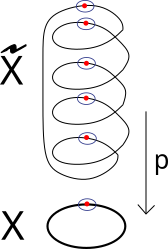
\includegraphics[scale=0.5]{./imagenes/spring.png}
  \end{figure}
  Ciertamente el intervalo \([0, 10 \pi]\) con \(0 \sim 10 \pi\) cumple
  el requisito, con el cubrimiento dado por
  \begin{align*}
    p : [0, 10 \pi] / _{(0 \sim 10\pi )} &\longrightarrow [0, 2 \pi] / _{(0 \sim 2\pi )} \\
    t &\longmapsto \mathrm t \mod 2 \pi
  \end{align*}
\end{ejemplo}
El diagrama anterior da una idea de la forma de general los espacios
cubrimientos \(\tilde X\), estos lucen como iteraciones del espacio base
\(X\). Por otro lado, sea \(x_0 \in S^1\) el punto rojo del diagrama, se
tiene la siguiente definicion auxiliad
\begin{definicion}[Fibra]
El conjunto discreto dado por \(p^{-1} (x_0)\) es conocido como una
\emph{fibra} de \(x_0\).
\end{definicion}
\noindent Una invariante interesante de este es que la cardinalidad de
cualquier fibra es la misma para todos los puntos.

\begin{ejemplo}[Cubrimiento de toro]
  En el ejemplo \ref{ej:toro-presentacion} se trabajo con la
  presentación de toro como espacio cociente de \([0,1]^2\). Siguiendo
  la idea del ejemplo anterior, podemos obtener un cubrimiento de esta
  presentación mediante el siguiente diagrama.
  \begin{figure}[h]
    \centering 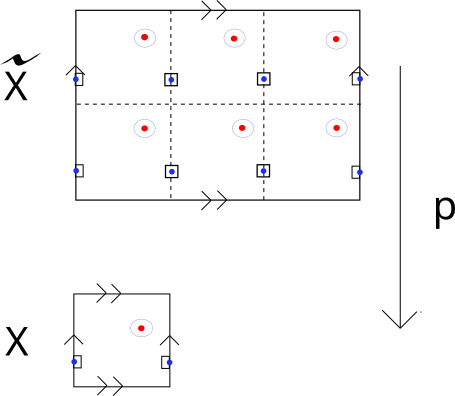
\includegraphics[scale=0.5]{./imagenes/toro-cubrimiento.png}
  \end{figure}
\end{ejemplo}

\begin{ejemplo}[Cubrimiento: \(\Re\) sobre \(S^1\)]
Para \(S^1\) el mapeo
\begin{align*}
  p : \Re &\longrightarrow S^1 \\
  t &\longmapsto e^{2 \pi \imath t}
\end{align*}
es claramente
sobreyectivo y continuo. Escogiendo dos abiertos ejemplares como \(U =
S^1 - \{(1,0)\}\) y \(V = S^1 - \{(-1,0)\}\), es claro que
\[
    p^{-1} (U) = \bigcup_{n \in \mathbb Z} (n, n+1)
    \qquad p^{-1} (V) = \bigcup_{n \in \mathbb Z} (n - \frac 1 2, n + \frac 1
    2 )
\]
Donde estas familias de conjuntos son disjuntos y restringidos a cada
uno se tiene la inyectividad requerida.
\end{ejemplo}

A priori el cubrimiento es independiente de los caminos que tengamos
en \(X\), queremos ver si podemos reflejar la información importante de
los caminos de \(X\) sobre \(\tilde{X}\);
\begin{figure}[h]
  \centering
  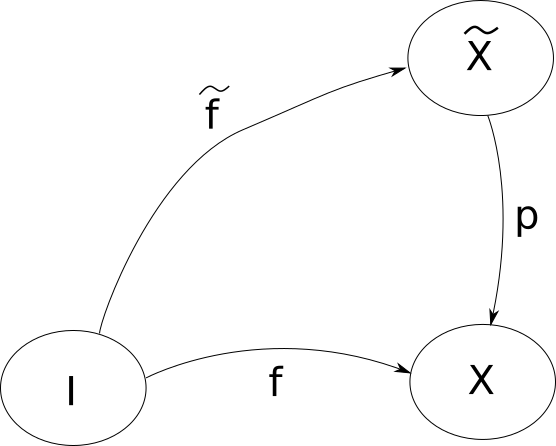
\includegraphics[scale=0.3]{./imagenes/lifting-path.png}
\end{figure}
es decir, para todo arco \(f : I \to X\), construiremos \(\tilde f : I
\to \tilde X\) el cual cumpla \(p \circ \tilde f = f \), donde \(\tilde
f\) sera nuestro representante en el espacio cubrimiento de este
camino. Veremos también que bajo ciertas hipótesis, este \(\tilde f\)
es único y refleja información homotopica. Para esto necesitamos
desarrollar algunos teoremas previos.
\begin{lema}[Numero de Lebesgue] \label{thm:lebesgue-number-lema}
  Sea \(\mathcal A\) un cubrimiento del espacio métrico \((X,d)\). Si
  \(X\) es compacto, entonces existe \(\delta > 0\) tal que para todo
  subconjunto de \(X\) teniendo diámetro menor que \(\delta\), existe un
  elemento de \(\mathcal A\) conteniéndolo.
\end{lema}
\begin{proof}
  Supongamos que \(X \not \in \mathcal A\), pues si no trivialmente el
  teorema se cumple \(\forall \delta > 0\). Por compacidad de \(X\)
  existe una colección \(\{A_1,\dotsc,A_n\} \subset \mathcal A\) que
  cubre a \(X\), definamos a los conjuntos \(C_i = X - A_i,\ \forall i
  \in [1,n]\) y a la función \(f : X \to \Re\) definida por
  \[ f(x) := \frac 1 n \sum_{i=1}^{n} d(x, C_i) \]
  i.e. la distancia promedio de \(x\) a \(C_i\). Notemos que \(\forall x
  \in X,\ f(x) > 0\), pues para \(x \in A_i \subseteq X\), por ser
  \(A_i\) un abierto, existe \(\epsilon > 0\) tal que \(B(x,\epsilon)
  \subset A_i\) y por tanto \(d(x, C_i) \geq \epsilon\) que implica \(
  f(x) \geq \frac \epsilon n > 0\).

  Por otro lado \(f\) es una función continua sobre \(X\) un espacio
  compacto, por lo tanto alcanza un mínimo; a este le denotaremos como
  nuestro \(\min_X f \coloneqq \delta \).

  Probaremos que este \(\delta\) cumple el requerimiento. Sea \(B
  \subset X\) subconjunto abierto de diámetro menor que \(\delta\), sea
  \(x \in B\) arbitrario. Escojamos el conjunto \(C_m\) como
  \[ C_m := \max_{i \in [1,n]} d(x, C_i) \]
  Dado que
  \[\delta \leq f(x) \leq d(x, C_m) \]
  Esto nos dice que dado \(\delta \leq d(x, C_m)\), existe una vecindad
  de al menos diámetro \(\delta\) que contiene a \(x\) en \(X - C_m = A_m\).
\end{proof}
\begin{definicion}[Levantamiento de \(f\)]
  Sea \(p : \tilde X \to X\) un mapeo. Si \(f : W \to X\) es un mapeo
  continuo, un levantamiento de \(f\) es una función \(\tilde f : W \to
  \tilde X\) tal que \(p \circ \tilde f = f\).
\end{definicion}
Ver que la definición es mucho mas general que lo que pedíamos al
diagrama. Usualmente \(W = [0,1]\) pues estudiaremos los caminos sobre
\(X\). Veremos a continuación teoremas de como se reflejan los caminos
y las homotopías en el espacio cubrimiento de \(X\).
\begin{teorema}[Levantamiento de caminos] \label{thm:lifting-theorem}
  Sea \(p : \tilde X \to X\) un cubrimiento y \(x_0 \in X\). Fijemos
  algún \(\tilde x _0 \in \tilde X\) tal que \(p(\tilde x _0) = x_0 \).
  Para cualquier camino \(f : [0,1] \to X\) que comience en \(x_0\), existe
  un único camino levantamiento \(\tilde f : [0,1] \to \tilde X\) tal que
  \(\tilde f (0) = \tilde x _0\)
\end{teorema}
\begin{proof}
  Para todo punto de \(x \in X\), existe una vecindad de este \(U_x\)
  que es cubierta (definicion \ref{def:cubierta}). Por tanto
  \[ X \subseteq \bigcup_{x \in X} U_x\]
  con \(U_x\) siendo las vecindades cubiertas para cada \(x\). De lo
  anterior, se obtiene la siguiente inclusion
  \[ [0,1] = f^{-1} \left( X \right) \subseteq f^{-1} \left( \bigcup_{x
    \in X} U_x \right) \]
  Por el Teorema \ref{thm:lebesgue-number-lema}, podemos elegir
  \(s_0,\dotsc,s_n \in [0,1]\) tal que para todo \(i \in \{0,1 \dotsc,
  n-1\}\), exista \(U_x\) tal que
  \[f \left( [s_i, s_{i+1}] \right) \subset U_x \]
  Con esto, definiremos \(\tilde f\) inductivamente.

  Primero declaremos \(\tilde f (0) = \tilde x _0\). Luego, suponiendo
  que \(\tilde f (s)\) esta definido para \(s \in [0, s_i]\), se
  define a \(\tilde f \) en \([s_i, s_{i+1}]\) de la siguiente forma.
  Dado que para algún \(x \in X\),
  \[
    f \left( [s_i, s_{i+1}] \right) \subseteq U_x \quad \land \quad
    \exists \{V_\alpha\}_{\alpha \in \Lambda},\ \bigcup_{\alpha \in \Lambda}
    V_\alpha = p^{-1} (U_x)
  \]
  debe de existir \(\alpha \in \Lambda\) tal que \(\tilde f (s_i) \in
  V_\alpha\) previamente definido; a este conjunto le denotaremos
  \(V_0\). Dado que \(p \mid_{V_0}\) es un homeomorfismo, definimos a
  \(\tilde f (s)\) en \([s_i, s_{i+1}]\) por
  \begin{equation} \label{eq:tilde-f-inductiva}
    \tilde f (s) = \left( p \mid _{V_0} \right)^{-1} \left( f(s) \right)
  \end{equation}
  El cual es continuo en \([0, s_i] \cup [s_i, s_{i+1}]\) en virtud del
  lema del pegamiento y bien definido por ser \( p \mid _{V_0} \)
  homeomorfismo.

  Para ver la unicidad, se probara inductivamente. Supongamos que existe
  otro \(\hat{f}\) levantamiento par de \(f\) que también
  comienza en \(x_0\), ie \(\hat{f} (0) = \tilde x _0 = \tilde f
  (0)\). Supongamos que que \(\forall s \in [0, s_i],\ \hat{f}
  (s) = \tilde f (s)\), dado que \(\tilde f\) esta definida por
  \eqref{eq:tilde-f-inductiva}, \(\hat f\) debe ser
  eventualmente diferente a la definición \eqref{eq:tilde-f-inductiva},
  pero
  \[\hat f (s_i) = \tilde f (s_i) \in V_0\]
  con \([s_i, s_{i+1}]\) conexo y la familia \(\{V_\alpha\}\)
  es disjunta, obliga\footnote{Funciones continuas mapean conjuntos
    conexos a conexos} a que
  \[ \hat f \left( [s_i, s_{i+1}] \right) \subset V_0 \]
  Dado que es un levantamiento, debe de cumplirse que
  \[\forall s \in [s_i, s_{i+1}],\ p \circ \hat f \, (s) =
    f(s) = p \circ \tilde f \, (s) \]
  \[ \iff p \left( \hat f (s) \right) = p \left( \left( p \mid_{V_0}
      \right) ^{-1} \left( f (s) \right) \right)\]
  \[ \implies \hat f (s) = (p \mid_{V_0})^{-1} (f (s)), \quad \forall s
      \in [s_i, s_{i+1}]\]
  siendo esta la única posible definición, pues de haber otra,
  se tendria una contradiccion en decir que \((p \mid_{V_0})\) es un
  homeomorfismo (mapeo único), por tanto se obliga a que \( \hat f =
  \tilde f\)
\end{proof}
Mas aun, podemos no solo levantar las curvas sobre \(X\) a \(\tilde X\),
si no también preservar las homotopías de \(X\) en \(\tilde X\).
\begin{corolario}[Levantamiento homotopico] \label{thm:levantamiento-homotopico}
  Sea \(p : \tilde X \to X\) un cubrimiento par tal que \(p(\tilde x _0)
  = x_0 \) para algún \(\tilde x _0 \in \tilde X\). Para cualquier
  función continua \(F : I \times I \to X\) tal que \(F(0,0) = x_0\), tiene una
  única función levantamiento continua \(\tilde F : I \times I \to
  \tilde X\) que cumpla \(\tilde F (0,0) = \tilde x_0\)
\end{corolario}
% Pagina 24 quitar referencias a la palabra par
\begin{proof}
  Lo único diferente con el teorema \ref{thm:lifting-theorem} es que
  tomamos \(I \times I\) que sigue siendo compacto. Podemos aplicar el
  teorema anterior primero definiendo \(\tilde F\) en \(0 \times I\),
  luego en \(I \times 0\) y escogiendo subdivisiones de \(I \times I\)
  \[ s_0 < s_1 < \dotsc < s_m \]
  \[ t_0 < t_1 < \dotsc < t_n \]
  tales que \(F ([s_i , s_{i+1}] \times [t_j \times t_{j+1}])\) este
  contenido en un conjunto cubierto en \(X\), esto utilizando
  el lema de Lebesgue al igual que en la demostración anterior.

  Luego definimos inductivamente \(\tilde F\) sobre \([s_i, s_{i+1}]
  \times [t_j , t_{j+1}]\) siempre y cuando \(\tilde F\) ya este
  definida sobre las lineas
  \[ L := [s_i , s_{i+1}] \times \{t_j\}\]
  \[ H := \{s_i\} \times [t_j , t_{j+1}] \]
  que son los bordes inferior y izquierdos del rectángulo.

  Tomamos el conjunto \(U\) par que contiene a la imagen
  \[ F([s_i , s_{i+1}] \times [t_j , t_{j+1}]) \subseteq U \subset X \]
  Por su paridad, podemos tomar la pre-imagen de \(p\) en \(U\) como
  \[ p^{-1}(U) = \bigcup_{\alpha \in \Alpha} V_\alpha\]
  Donde la familia \(\{V_\alpha\}\) es disjunta.

  Dado que \( \{(s_i, t_j)\} = L \cap H\) y que \( (s_i , t_j) \) ya
  esta definido bajo \(\tilde F\), existe un único \(V_0 \in
  \{V_\alpha\}\) que contiene a \(F (s_i, t_j)\). Pero notando que
  \(\{V_\alpha\}\) son disjuntos y que \(L,H\) son conexos, obliga a que
  \[ \tilde F (H) \subset V_0, \quad \tilde F (L) \subset V_0 \]
  Luego podemos definir \(\tilde F\) sobre el resto de \([s_i,
    s_{i+1}] \times [t_j , t_{j+1}]\) notando que \(p \mid_{V_0}\) es
  un homeomorfismo entre \(V_0\) y \(U\) y por tanto
  \[ \forall (a,b) \in [s_i, s_{i+1}] \times [t_j , t_{j+1}],
    \ \tilde F (a,b) := p^{-1} \mid_{V_0} \left( F(a,b) \right) \]
  Esta cumple la regla \( F = p \circ \tilde F\) y es continua en virtud
  del lema del pegamiento. Notando finalmente que ahora los conjuntos
  \[ L := [s_i , s_{i+1}] \times \{t_{j+1}\}\]
  \[ H := \{s_{i+1}\} \times [t_j , t_{j+1}] \]
  Están definidos en \(\tilde F\) y pueden ser utilizados para seguir
  definiéndola inductivamente sobre \(I \times I\).
%fin pagina 24
\end{proof}

Retrocedamos un poco para pensar que es lo que tenemos hasta el momento.
Para un cubrimiento \(p : \tilde X \to X\), siempre es valida la
construcción de la definición \ref{def:homomorfismo-inducido} de un
hilomorfismo inducido \(p_* : \pi \left( \tilde X , \tilde x _0 \right)
\to \left( X , x_0 \right)\) con \(p (\tilde x_0) = x_0\). Pero a priori
esto no nos da ninguna relación entre contención entre los grupos. Pero
cuando \(p\) es un cubrimiento, tenemos que \(p_*\) es inyectiva por el
siguiente teorema.

\begin{teorema}[Inyectividad de homomorfimos inducido por cubrimientos]
  Sea \(\left( \tilde X, \tilde x_0 \right), \left( X, x_0 \right)\)
  dos espacios topológicos puntuados. Si \(p : \left( \tilde X, \tilde x_0
  \right) \to \left( X, x_0 \right)\) un cubrimiento entre estos,
  entonces el homomorfismo inducido
  \[ p_* : \pi \left( \tilde X, \tilde x_0 \right) \longrightarrow \pi
    \left( X, x_0 \right)\]
  es inyectivo.
\end{teorema}
\begin{proof}
  Que el homomorfismo \(p_*\) sea inyectivo equivale a que su
  kernel sea únicamente la identidad. Para esto
mostraremos que todo elemento \([\tilde f] \in \pi
(\tilde X , \tilde x_0)\) tal que \(p_* ([\tilde f]) = [k_{x _0}]\) con \([k_{ x _0}]\)
la identidad de \(\pi (X, x_0)\), esta obligado a cumplir \([\tilde f] =
[k_{\tilde x _0}]\) donde \([k_{\tilde x _0}]\) es la identidad de \(\pi (\tilde X ,
\tilde x _0)\).

Sea \([\tilde f] \in \pi (\tilde X, \tilde x _0)\) un elemento
arbitrario tal que
\[p_* ([\tilde f]) = [p \circ \tilde f] = [k_{ x _0}]\]
Esto equivale a decir que existe una homotopía \(H\) entre \(p_* \circ
f\) y \(k_{x _0}\). Por el corolario \ref{thm:levantamiento-homotopico} podemos
levantar esta homotopía \(H\) en \((X, x_0)\) a una homotopía
levantamiento \(\tilde H\) en \((\tilde X , \tilde x _0)\). Esta es un
levantamiento homotópico, por tanto cumple la ecuaciones
\[ p \circ \tilde H = H, \quad H (t, 0) = p \circ \tilde f, \quad H (t,
  1) = k_{x _0} \]
por lo que \(\tilde H\) es una homotopía entre los levantamientos de \(p
\circ \tilde f\) y \(k_{x _0}\). Por el teorema \ref{thm:lifting-theorem},
sabemos que estos levantamientos son únicos. También sabemos por simple
calculo que
\[ p \circ k_{\tilde x _0} (t) = p \left( \tilde x_0 \right) = x_0 =
  k_{x_0} (t) ,\quad \forall t \in [0,1] \]
por lo que \(k_{\tilde x _0}\) es el levantamiento de \(k_{x_0}\).
Además de ya conocer que \(\tilde f\) es el levantamiento de \(p \circ
\tilde f\). Por tanto \(\tilde H\) es una homotopía entre \(\tilde f\) y
\(k_{\tilde x _0}\) ie
\[[\tilde f] = [k_{\tilde x_0}]\]
obteniendo así que el kernel de \(p_*\) es trivial.
\end{proof}

Hemos mostrado que para un cubrimiento \(p : (\tilde X, \tilde x _0) \to
(X , x_0)\), se tiene que
\[ \pi (\tilde X, \tilde x_0) \simeq p_* \left( \pi (\tilde X, \tilde x_0)\right) \]
donde \(p_* \left( (\tilde X, \tilde x_0) \right)\) es un subgrupo de
\(\pi (X, x_0)\). Con esto podemos revisar algunos ejemplos anteriores.
\begin{ejemplo}[Ejemplo \ref{ej:10pi} continuado]
  En el ejemplo anterior se había definido \(p : [0 , 10 \pi] /_{0 \sim
    10\pi} \to [0, 2\pi] /_{0 \sim 2\pi}\).
  \begin{figure}[h]
    \centering 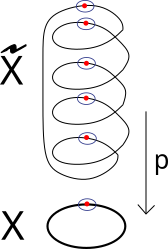
\includegraphics[scale=0.5]{./imagenes/spring.png}
  \end{figure}
  Consideremos a \(x_0 \in [0, 2\pi] /_{0 \sim 2\pi}\) un punto base. El
  homomorfimos inducido para \(p\) corresponde a la función
  \begin{align*}
    p_* : \pi \left( [0, 2\pi] /_{0 \sim 2\pi} , x_0 \right) &\longrightarrow \left( [0, 10\pi] /_{0 \sim 10\pi}, x_0 \right) \\
    [f] &\longmapsto [p \circ f]
  \end{align*}
  Según el diagrama, el claro ver que ambos grupos solo admiten una
  curva no trivial en ellos. Llamaremos
  \begin{gather*}
    [\gamma] \in \pi \left( [0, 10\pi] /_{0 \sim 10\pi}, x_0 \right),\
    \gamma (t) := 10 \pi t \\
    [\alpha] \in \pi \left( [0, 2\pi] /_{0 \sim 2\pi}, x_0 \right), \
    \alpha (t) := 2 \pi t
  \end{gather*}
  a estas. Calculando la imagen de \([\gamma]\) bajo \(p_*\) se obtienen
  las siguiente ecuaciones
  \begin{equation*}
    p_* \left( [\gamma] \right) = [p \circ \gamma]
  \end{equation*}
  donde
  \[
    p \circ \gamma (t) = 10 \pi t \mod 2 \pi = \alpha^5
  \]
  luego, reemplazando en la ecuación anterior
  \begin{equation*}
    p_* \left( [\gamma] \right) = [p \circ \gamma] = [\alpha^5] =
    [\alpha]^5
  \end{equation*}
  Dado que \(p_*\) es un homomorfismo, es claro que \(p_* \left(
  [\gamma]^n \right) = [\alpha]^{5n}\). Conociendo que \(\pi \left(
  [0,2\pi] /_{0 \sim 2\pi} , x_0 \right)\) es \((\mathbb Z, +)\) es claro
  ver que \(p_* \left( \pi \left( [0, 10\pi] , x_0 \right) \right)\) es
  \(5 \mathbb Z \) que es isomorfo (ambos tienen un unico generador) a
  \(\mathbb Z\).
\end{ejemplo}

Una pregunta ha hacerse es si tenemos esta implicación
en sentido contrario, si todo subgrupo de \(\pi(X, x_0)\) le corresponde
un cubrimiento el cual cumpla esta relación. La respuesta es afirmativa.
La demostración no es nuestro enfoque, pero se invita a los interesados
en revisar el teorema 1.3.6 de Hatcher \cite{Hatcher}.

% eliminar?
Ahora es mas clara la forma de calcular grupos fundamentales usando
cubrimiento. Si tuviéramos de partida un isomorfismo de grupos
entre los espacios \(\pi (\tilde X)\) y \(\pi (X)\), tendríamos que
presuponer la estructura del grupo en \(\pi (\tilde X)\). La alternativa
presentada muestra que los cubrimientos, preservan los arcos y
homotopías de \(X\) en \(\tilde X\) y si es el espacio \(\tilde X\) es
suficientemente simple como para admitir un calculo simple de su grupo
fundamental, entonces podemos saber que el grupo de \(X\) es un subgrupo
normal del grupo de \(\tilde X\).

Para un calculo mas explicito necesitamos denotar los puntos finales
obtenidos en \(\tilde X\).
\begin{definicion}[Levantamiento derivado]
  Sea \(p : \tilde X \to X\) un cubrimiento y sea \(x_0 \in X\).
  Escojamos \(\tilde x _0 \in \tilde X\) tal que \(p(\tilde x _0) =
  x_0\). Dado un elemento \([f] \in \pi (X, x_0)\), sea \(\tilde f\) el
  levantamiento (único) de \(f\) a un camino en \(\tilde X\) que
  comienza en \(\tilde x _0\). Definamos \(\phi ([f]) = \tilde f (1)\) del
  \(\tilde f\) asociado a \(f\) anteriormente. Entonces \(\phi\) es bien
  definido como mapeo de conjunto
  \[ \phi : \pi (X, x_0) \longrightarrow p^{-1} (x_0)\]
  llamando a \(\phi\) el \textbf{correspondiente levantamiento
  derivado}\footnote{Corresponding lifting path} del cubrimiento \(p\).
\end{definicion}
La definición anterior intuitivamente ``desenrolla'' los ciclos del
grupo fundamental \(\pi (X,x_0)\) y ve donde terminan vistos sobre
\(\tilde X\).
\begin{teorema}
  Sea \(p : \tilde X \to X\) un cubrimiento tal que \(p (\tilde x _0) =
  x_0\). Si \(\tilde X\) es arco-conexo entonces el correspondiente
  levantamiento \(\phi : \pi (X, x _0) \to p^{-1} (x_0)\) es
  sobreyectivo. Mas aun, si \(\tilde X\) es simplemente conexo, este es
  biyectivo.
\end{teorema}
Usualmente queremos que \(p^{-1} (x)\) no sea simplemente un conjunto,
queremos poder dotarle de estructura de grupo. En caso de \(\tilde X\)
ser arco-conexo, lo que estamos haciendo realmente es estudiar un
subgrupo de \(\pi \left( X, x_0 \right)\) a través de \(p^{-1}(x_0)
\subseteq \tilde X\).
\begin{proof}
  Demostración estándar de sobreyectividad en caso de ser \(\tilde X\)
  arco-conexo. Para \(\tilde x _1 \in p^{-1} (x_0)\) arbitrario, existe
  \(\tilde f\) camino entre \(\tilde x _0 \) a \(\tilde x _1\) por
  arco-conexidad. Definimos \(f := p \circ \tilde f\), el cual es un
  camino \(f : I \to X\) que cumple \(\phi ([f]) = \tilde x _1\) por
  definición.

  En caso de ser \(\tilde X\) simplemente-conexo, veremos solo la
  inyectividad. Sean \([f],[g] \in \pi (X, x_0)\) tales que \(\phi([f])
  = \phi([g])\), mostraremos que \([f] = [g]\). Sean \(\tilde f, \tilde
  g : I \to \tilde X\) los levantamientos respectivos que comienzan en
  \(\tilde x _0\). Dado que \(\phi([f]) = \tilde f (1) = \tilde g (1) =
  \phi([g])\) y la simple-conexidad de \(\tilde X\), existe \(\tilde F :
  I \times I \to \tilde X\) homotopía \(\tilde f, \tilde g\). Luego \(p
  \circ \tilde F : I \times I \to X \) es una homotopía entre \(f, g\),
  por tanto \([f] = [g]\)
\end{proof}
Ahora podemos plantearnos un ejemplo clásico, ver el grupo fundamental
de \(S^1\). Utilizaremos el teorema anterior para proponer un
cubrimiento tal que \(\tilde X\) sea simplemente conexo y que pueda
preservar la estructura de grupo para ser estudiado bajo ese lente.
\begin{teorema} \label{thm:grupo-S1}
  \(\forall x_0 \in S^1,\ \big( \pi (S^1,x_0), * \big)\) es isomorfo a
  \((\mathbb Z, +)\)
\end{teorema}
\begin{proof}
  Dado que \(S^1\) es arco-conexo, basta probar que este teorema es
  cierto para algún \(x_0\) en \(S^1\). Sea \(p : \mathbb R \to S^1,\
  p(t) := (\cos 2 \pi t, \sin 2 \pi t)\) el cual es fue visto anteriormente
  que es un cubrimiento par. Sea \(\tilde x _0 = 0\) y \( p(\tilde x _0) =
  (1,0) =: x_0 \in S^1\). Por ser \(\mathbb R\) simplemente conexo, se
  tiene que el levantamiento correspondiente \(\phi : \pi (S^1, x_0) \to
  p^{-1} (x_0)\) es biyectivo, donde
  \[ p^{-1} (1,0) = \{t \in \mathbb R \mid (\cos 2 \pi t, \sin 2 \pi t)
    = (1, 0) \} = \mathbb Z \]
  Notamos además que de sobre todo \(\mathbb Z\) existe únicamente el
  grupo bajo la adición, este sera nuestro grupo de partida.

  Para probar que es homomorfismo, se toman \([f], [g] \in \pi
  (S^1, x_0)\) arbitrarios y \(\tilde f, \tilde g\) sus correspondientes
  levantamientos tales que \(n := \tilde f (1) = \phi ([f]),\ m :=
  \tilde g (1) = \phi ([g])\). Ahora queremos encontrar quien es el
  levantamiento de \([f] * [g]\), para esto se define el camino
  \begin{align*}
    \tilde{\tilde g} : I &\longrightarrow \mathbb R \\
    s &\longmapsto n + \tilde g (s)
  \end{align*}
  Puesto que \(p(n + x) = p(x)\) por periodicidad, se cumple que
  \[ p \circ \tilde{\tilde g} (x) = p (n + \tilde g (x)) = p (\tilde g
    (x)) = g (x) \]
  Por tanto \(\tilde{\tilde g}\) es el levantamiento de \(g\) para
  \(\tilde x_0 = n\) (en vez de \(\tilde x_0 = 0\)). Luego el producto
  \(\tilde f * \tilde{\tilde g}\) esta bien definido pues \(\tilde f (1)
  = n = \tilde{\tilde g} (0)\) y se afirma que este es el levantamiento
  de \(f * g\) pues por calculo
  \[ p \circ (\tilde f * \tilde{\tilde g}) =
     ((p \circ \tilde f) * (p \circ \tilde{\tilde g})) =
     (f * g)
  \]
  Por ultimo calculamos
  \[ \phi ([f] * [g]) = \tilde{\tilde g} (1) = n + m = \phi ([f]) + \phi
  ([g]) \]
  Por lo que \(\phi\) es un homomorfismo de grupos.
\end{proof}

\paragraph{Ejemplo: Cubrimiento \(p_n : S^1 \to S^1\).} Para testear la intuición
de que el espacio cubrimiento refleja en el caso común un subgrupo del
espacio topológico, tomemos el caso
\begin{align*}
  p_n : S^1 &\longrightarrow S^1 \\
  z &\longmapsto z^n
\end{align*}
Para este, nuestro conjunto \(p^{-1} (x_0)\), con \(x_0 = (1,0)\) se
obtiene mediante la reducción
\begin{align*}
  p^{-1} (1,0)
    &= \{ z \in S^1 \mid z^n = (1,0)\} \\
    &= \{z \in S^1 \mid (\cos 2 \pi n t, \sin 2 \pi n t) = (1,0) :
           t \in [0,1] \} \\
    &= \{(\cos 2 \pi t, \sin 2 \pi t) \in S^1 \mid
           t \in \{0, \frac 1 n , \dotsc , \frac {n-1} n \} \}
\end{align*}
\[ \therefore p^{-1}(1,0) \simeq \mathbb Z / n \mathbb Z \]
Además bajo el mismo tratamiento utilizado anteriormente en \(\pi (S^1,
x_0) = \mathbb Z\) para \(\phi\), este es un homo-morfismo. Esto muestra
que la elección de \(p\) afecta que subgrupo de \(\pi (S^1, x_0)\) estudiaremos.
\begin{teorema}
  Sea \(p : \tilde X _1 \to X_1,\ p' : \tilde X _2 \to X_2 \) dos
  cubrimientos pares, entonces
  \[ p_1 \times p_2 : \tilde X _1 \times \tilde X _2 \to X_1 \times X_2 \]
  Es un cubrimiento par.
\end{teorema}
\begin{proof}
  Para todo \(x_1 \in X_1,\ x_2 \in X_2\), existen \(U_1, U_2\)
  vecindades pares respectivamente tales que son cubiertas por \(p_1,
  p_2\). Denotemos a \(\{V_\alpha^{(1)}\}, \{V_\beta^{(2)}\}\) familias
  de conjuntos tales que
  \[
    \begin{matrix}
      \bigcup_{\alpha} V_\alpha^{(1)} = p_1^{-1} (U_1) &
      \bigcup_{\alpha} V_\alpha^{(2)} = p_2^{-1} (U_2)
    \end{matrix}
  \]
  \[ \bigcup_{\alpha, \beta} V_\alpha^{(1)} \times V_\beta^{(2)} = (p_1
    \times p_2)^{-1} (U_1 \times U_2)\]
  Donde la restricción a un \(V_{\bar{\alpha}}^{(1)} \times
  V_{\bar{\beta}}^{(2)}\) arbitrario en \(p_1 \times p_2\) obtiene un
  homeomorfismo en virtud de las componentes.
\end{proof}

Esto es una extensión del resultado que ya conocíamos sobre el functor
entre \(\mathbf{HoTop}_{*}\) y \(\mathbf{Grp}\) en cuanto a preservación
del producto. Esto no dice que el ``calculo'' de grupos fundamentales
también puede derivarse del conocimiento del productor de cubrimientos
pares.

\paragraph{Ejemplo Toro en \(R^4\).} Dado que podemos caracterizar al
toro \(T^1\) como \(S^1 \times S^1\), el teorema anterior nos dice que
\((\pi (T^1, b), *) = (\pi (S^1, b) \times \pi (S^1, b), *) = (\mathbb Z
\times \mathbb Z, +) \)
\subsection{Teorema de \vank}
Este teorema es considerado como el mas útil a la hora de hacer
identificaciones de grupos fundamentales. Su idea se basa en que si
tenemos un espacio \(X\) y dos subconjuntos \(U,V\) tales que \(X = U
\cup V\), entonces podemos estudiar el grupo \(\pi (X, x_0)\) como un
subgrupo del grupo libre generado por \(\pi (U, x_0)\) y \(\pi (V,
x_0)\). Para obtener un isomorfismo tomamos un cociente adecuado. El
caso mas claro de aplicación se vera que son para las \emph{wedge sum}
en donde este cociente sera trivial. En casos mas generales se vera que
el cociente es de una forma relacionada con la definición de producto
libre. Procedemos para iniciar la definición de estos conceptos.

\begin{definicion}[Producto libre]
  Sea \(G_\alpha\) una colección de grupos. El grupo libre \(*_\alpha
  G_\alpha \) consiste como conjunto en todas las cadenas reducidas
  \[ g_1 g_2 g_3 \dots g_m \]
  para \(m \geq 0\) arbitrario tal que todo \(g_i\) pertenece a
  \(G_{\alpha_i}\), \(g_i\) distinto de la identidad de
  \(G_{\alpha_i}\) y índices sucesivos son distintos, ie \(\alpha_i \neq
  \alpha_{i + 1}\). Tomando la identidad como la cadena vacía y como
  operación de grupo la juxtaposicion de cadenas
  \[ (g_1 g_2 \dots g_m ) \cdot (h_1 h_2 \dots h_l) = g_1 g_2 \dots g_m
    h_1 h_2 \dots h_l \]
  en donde se debe reducir la cadena para que términos seguidos no
  pertenezcan al mismo grupo.
\end{definicion}
\begin{acotacion}
  Es claro que la cadena vacía es la identidad. Para ver la inversa de
  una cadena nos basamos en el proceso de reducción. Sea \(g_1 g_2 \dots
  g_m\) una cadena arbitraria, su inversa corresponde a \(g_m^{-1} g_{m-1}^{-1}
  \dots g_1^{-1}\) pues
  \begin{gather*}
    g_1 g_2 \dots g_{m-1} \underbrace{g_m g_m^{-1}}_{= e_{\alpha_m}}
      g_{m-1}^{-1} \dots g_1^{-1} \\
    = g_1 g_2 \dots g_{m-1} g_{m-1}^{-1} \dots g_1^{-1}
  \end{gather*}
  donde la identidad fue removida de la cadena por el requisito de ser
  una cadena reducida. Si este proceso continua iterativamente se
  obtendrá la cadena vacía que es la identidad.

  Por otro lado se nota que no hay requerimiento de que todos los grupos
  participen en todas las cadenas. De hecho, todos los elemento de
  cualquiera de los grupos participantes \(G_\alpha\) pertenecen al
  conjunto de cadenas reducidas como cadenas con \(m = 1\) y índice
  adecuado.
\end{acotacion}
Esta construcción puede considerarse como una alternativa a \(\prod
G_\alpha\) o \(\oplus G_\alpha\) en donde elementos de distintos grupos
no conmuten entre si. Como ejemplo podemos tomar a \(\mathbb Z * \mathbb
Z\) con cada \(\mathbb Z\) con su propio generador, a los cuales
denotaremos por \(a\) y \(b\) respectivamente. Este corresponde al grupo
de la cadenas \(a^{n_1} b^{n_2} a^{n_3} \dots a^{n_m}\) con \(n_i \in
\mathbb Z \). Algo que no es claro sobre este grupo es si
su operación es asociativa, esto lo probaremos en el siguiente teorema
por completitud
\begin{teorema}
  El producto de \(*_\alpha G_\alpha\) es asociativo.
\end{teorema}
\begin{proof}
  Mostrar directamente la asociatividad del producto seria un ejercicio
  de enumerar los casos donde puede ocurrir un reducción de cadena.
  Nosotros seguiremos una vía alternativa dada por \emph{Hatcher} en
  \cite{Hatcher}[sec 1.2] de estudiar la cada posible juxtaposicion como
  una función en el espacio de permutaciones. Sea \(W\) el conjunto de
  cadenas reducidas de \(*_\alpha G_\alpha\) con la cadena vacía
  incluida. Para cada \(g \in G_\alpha\) se define una función asociada
  \(L _g : W \to W\) dada por la ecuación
  \[ L_g \left( g_1 g_2 \dots g_m \right) = g g_1 g_2 \dots g_m \]
  con \(g g_1\) reducido si \(g_1 \in G_\alpha \) para mantener que sea
  una cadena reducida en \(W\). Una propiedad clara es que podemos
  simplificar en \(G_\alpha\) antes o después de asociar \(L\) y no
  afectara el resultado, dicho formalmente sea \(g, g', \hat g \in
  G_\alpha\) con \(\hat g = g \cdot g'\). La asociación \(L_{g \cdot
  g'}\) cumple que \(L _{g \cdot g'} = L_{g} \circ L_{g'}\) pues para una
  cadena arbitraria
  \begin{align*}
    &L_{g \cdot g'} \left( g_1 g_2 \dots g_m \right) \\
    &= (g \cdot g') (g_1 g_2 \dots g_m) \\
    &= (\hat g) (g_1 g_2 \dots g_m) \\
    &= (g (g' (g_1 g_2 \dots g_m))) \\
    &= L_g \circ L_{g'} \left( g_1 g_2 \dots g_m \right)
  \end{align*}
  notando de que en el caso que \(g_1 \in G_\alpha\) se tiene un
  reducción intermedia. Se ve también de todo \(L_g\) con \(g \in
  G_\alpha\) tiene una asociada inversa \(L_{g^{-1}}\) con \(g^{-1} \in
  G_\alpha\), lo cual en consecuencia nos da un mapeo de identidad a
  identidad (por regla de reducción). Por lo anterior tenemos un
  homomorfismo de grupos entre \(G_\alpha\) y \((W \to W, (\circ))\) y
  esto para todo \(\alpha\).
  \begin{align*}
    L: G_\alpha &\longrightarrow P(W) \\
    g &\longmapsto L_g
  \end{align*}

  Podemos de generalizar \(L\) en su primer
  argumento de \(G_\alpha\) con \(\alpha\) arbitrario a todo \(W\). Esto
  se hace por la siguiente formula
  \begin{align}
    \hat L : W &\longrightarrow P(W) \nonumber \\
    g_1 g_2 \dots g_k &\longmapsto L_{g_1} \circ L_{g_2} \circ \dots
    \circ L_{g_k} \label{def:hatL}
  \end{align}
  Una propiedad de \(\hat L\) es que es inyectiva, esto se ve notando
  que las únicas cadenas que mapean bajo \(\hat L\) a la identidad de
  \(P (W)\) corresponden a la cadena vacía o a las identidades de los
  distintos \(G_\alpha\) que por definición no pertenecen a \(W\).

  Ahora podemos ver la asociatividad de \(W\) con la yuxtaposición. Sea
  \(w_1, w_2, w_3 \in W\) tres cadenas tales que \(w_1 (w_2 w_3) \neq
  (w_1 w_2) w_3\). Estudiamos \[\hat L_{w_1 (w_2 w_3)},\ \hat L_{(w_1
    w_2) w_3}\] que por ecuación \eqref{def:hatL} corresponde a la
  composición de varias funciones \(L_g\) con \(g\) elementos de las
  cadenas \(w_1, w_2, w_3\).  No es difícil ver que en ambas expansiones
  participan las mismas funciones \(L_g\) y en el mismo orden. Mas aun,
  dado que la composición en \(P(W)\) es asociativa, nos estaría diciendo
  que
  \[ \hat L_{w_1 (w_2 w_3)} = \hat L_{(w_1 w_2) w_3}\]
  Pero dado que \(\hat L\) es inyectiva, esto implica que \(w_1 (w_2
  w_3) = (w_1 w_2) w_3\). Dada que estas cadenas son arbitrarias,
  estamos diciendo que \(W\) con la yuxtaposición (ie \(*_\alpha
  G_\alpha\)) es asociativo.
\end{proof}

Aquí se utilizo implícitamente un propiedad básica del producto libre
\(*_\alpha G_\alpha\), que si tengo una colección de homomorfismos
\[ \phi_\alpha : G_\alpha \to H \]
con \(H\) un grupo, existe una extensión única
\[ \phi : *_\alpha G_\alpha \to H \]
tal que sigue siendo homomorfismo. En particular, la ecuación que la
define para \(g_1 g_2 \dots g_n \in *_\alpha G_\alpha\) arbitrario es la siguiente
\[
  \phi \left( g_1 g_2 \dots g_n \right) := \phi_{\alpha_1} (g_1)
  \phi_{\alpha_2} (g_2) \dots \phi_{\alpha_n} (g_n)
\]
Para probar que es única, basta notar reducir la cadena no afecta la
imagen bajo \(\phi\) y que esta debe seguir siendo un homomorfismo.

El marco de trabajo de \vank sera el siguiente diagrama conmutativo,
\begin{figure}[h]
  \centering
  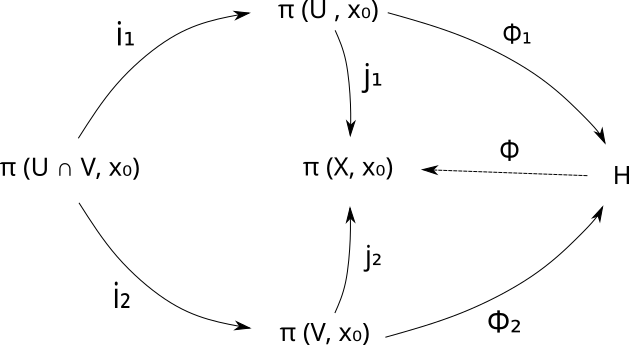
\includegraphics[scale=0.5]{./imagenes/van.png}
\end{figure}
donde \( H = \pi (U, x_0) * \pi (V, x_0)\) el producto libre, \(i_1,
i_2, j_1, j_2\) son los homomorfismos inducidos (sin la notación \(i_*\)
por simplicidad) de las inclusiones correspondientes, \(\Phi_1, \Phi_2\)
son las inclusiones en el grupo libre tomando todo \(\gamma \in \pi (U,
x_0)\) y ver la correspondiente cadena \(\gamma \in H\) y \(\Phi :
\pi(U, x_0) * \pi (V, x_0) \to \pi (X, x_0)\) la extensión de los
homomorfismo \(\Phi_1, \Phi_2\) descrita en el párrafo anterior.

Previo al teorema general, es útil trabajar con una versión reducida del
teorema de \vank por dos razones: es una versión geométricamente
intuitiva y aparece como paso intermedio de la demostración general.

\begin{teorema} \label{thm:vank-especifico}
  Sea \(X = U \cup V\), donde \(U,V\) son conjuntos abiertos de \(X\).
  Supongamos que \(U \cap V\) es arco-conexo y que \(x_0 \in U \cap V\).
  Sea \(j_1\) y \(j_2\) las inclusiones de \(U\) y \(V\) en \(X\)
  respectivamente. Entonces las imágenes de los homomorfismos inducidos
  \[ j_{1,*} : \pi (U, x_0) \to \pi (X, x_0), \quad j_{2,*} : \pi
  (V, x_0) \to \pi (X, x_0) \]
  generan a \(\pi (X,x_0)\).
\end{teorema}
\begin{proof}
  Hemos de probar que para todo arco \(f\) en \(X\) basado en \(x_0\),
  es arco-homotópico a un arco de la forma
  \[ g_1 * g_2 * ... * g_n \]
  donde cada \(g_i\) es un arco en \(X\) basado en \(x_0\) que esta
  contenido completamente en \(U\) o en \(V\).

  Por el lema \ref{thm:lebesgue-number-lema} (numero de Lebesgue),
  existe una subdivisión de \(I\) dada por
  \[ 0 = a_0 < ... < a_n = 1\]
  tal que
  \(f ([a_i , a_{i+1}])\) pertenece completamente a \(U\) o \(V\) para
  todo \(i \in \{1 \dotsc n\}\). Si para para todo \(i\) se cumpliera que
  \(f(a_i) \in U \cap V\) hemos terminado. En caso contrario, de existir
  \(i\) tal que \(f(a_i) \not \in U \cap V\) esto implica que
  \[ f(a_i) \in U \ \veebar \ f(a_i) \in V \]
  Tomando s.p.d.g la primera alternativa, implicaría que
  \[ f(a_i) \in U \implies f([a_{i-1}, a_{i}]) \subset U \ \land \ f([a_i,
    a_{i+1}]) \subset U \]
  análogamente si \(f(a_i) \in V\). Podemos olvidar entonces el valor
  \(a_i\) de la subdivisión y revisar si \(f(a_{i+1}) \in U \cap V\),
  repitiendo este proceso una cantidad finita de veces hasta satisfacer
  la condición.

  Ahora se prueba el teorema en si. Dado \(f\) y \(a_0 < ... < a_n\)
  subdivisión anterior, definamos las funciones
  \[ l_i : [0,1] \to [a_{i-1}, a_{i}] \]
  \[ f_i = f \circ l_i \]
  Es claro que \(\forall i \in \{1 \dotsc n\}, \ f_i (I) \) esta contenida en
  \(U\) o en \(V\). También es claro por simple calculo que se cumple
  la igualdad
  \[ [f] = [f_1] * [f_2] * ... * [f_n] \]
  Pero estos \(\{f_i\}\) no son arcos cerrados basados en \(x_0\) de
  \(\pi (U,x_0)\) o \(\pi (V,x_0)\). Para solucionar esto, nos basamos
  en la arco conexidad de \(U \cap V\), lo que nos permite afirmar que
  para todo \(i \in [1 , n]\) existe
  \[ \alpha_i : I \to U \cap V \]
  \[ \alpha_i (0) = x_0, \quad \alpha_i (1) = f(a_i) \]
  arcos continuos, fijando además \(\alpha_0 \equiv x_0 \equiv \alpha_n
  \). Estos nos permiten construir los arcos
  \[ g_i = \alpha_{i-1} * f_i * \alpha_i^{-1} \]
  los cuales si están basados en \(x_0\), y cuya imagen sigue estando
  contenida en \(U\) o en \(V\). Por simple calculo se ve que
  \[ [g_1] * ... * [g_n] = [f_1] * ... * [f_n] = [f] \]
\end{proof}
\begin{corolario}\label{cor:sobre-van}
  El homomorfismo \(\Phi : \pi (U, x_0) * \pi (V, x_0) \to \pi (X,
  x_0)\) es sobreyectivo.
\end{corolario}
\begin{proof}
  En el final de la demostración anterior, la cadena \(g_1 g_2 \dots
  g_n\) tiene como imagen bajo \(\Phi\) a \([f]\) pues
  \[ \Phi \left( g_1 g_2 ... g_n \right) = [g_1] * [g_2] * ... *
    [g_n] = [f] \]
  Dado que este \([f]\) era un elemento arbitrario de \(\pi \left( X,
    x_0 \right)\), tenemos lo afirmado.
\end{proof}
Uno puede generalizar el teorema anterior para una cantidad arbitraria
de conjuntos \(A_\alpha\) tal que \(X = \bigcup A_\alpha\). La
demostración es la misma, solo tal vez un poco mas difícil de
visualizar. Lo importante de este teorema es el corolario, el cual
utilizaremos en su forma generalizada para probar el teorema general.

\begin{teorema}[\vank]
  Sea \((X, x_0)\) un espacio puntuado tal que exista una familia de
  conjuntos \(\{A_\alpha\}_{\alpha \in \tau}\) la cual cumpla que todo
  elemento de esta contiene a \(x_0\) y \( X = \bigcup_{\alpha \in \tau} A_\alpha\). Si para cada
  intersección \(A_\alpha \cap A_\beta\) es arco-conexa, entonces el
  homomorfismo
  \[ \Phi : *_\alpha \pi (A_\alpha, x_0) \to \pi (X, x_0) \]
  es sobreyectivo.

  Mas aun, si cada intersección \(A_\alpha \cap A_\beta
  \cap A_\gamma\) con \( \alpha, \beta, \gamma \in \tau\) es arco-conexa,
  entonces el kernel de \(\Phi\) es un subgrupo normal \(N\) de la forma
  \[
    N := N \left( \{ i_{\alpha \beta} (\omega) i_{\beta \alpha} (\omega)^{-1}
    \mid \omega \in \pi \left( A_\alpha \cap A_\beta, x_0 \right),\
    \forall \alpha ,\beta \in \tau \} \right)
  \]
  es decir el subgrupo normal generado por estos elementos y por tanto
  \(\Phi\) induce un isomorfismo \(\pi (X, x_0) \cong *_\alpha \pi
  (A_\alpha, x_0) / N \)
\end{teorema}
Antes de la demostración hablaremos un poco del conjunto \(N\). Las
funciones \(i_{\alpha \beta}, i_{\beta, \alpha}\) corresponden a los
homomorfismos inducidos por la inclusión
\begin{gather*}
  i_{\alpha \beta} : \pi (A_\alpha \cap A_\beta , x_0 ) \longrightarrow \pi (A_\alpha, x_0) \\
  i_{\beta \alpha} : \pi (A_\alpha \cap A_\beta , x_0 ) \longrightarrow \pi (A_\beta, x_0)
\end{gather*}
que pierden su notación \(i_*\) por simplicidad. Notar que
para \(\omega \in \pi (A_\alpha \cap A_\beta ,\ x_0)\) arbitrario
\[ i_{\alpha \beta} (\omega) i_{\beta \alpha}^{-1} (\omega) \in N
  \implies i_{\alpha \beta} (\omega) \cdot N = i_{\beta
\alpha} (\omega) \cdot N \]
con \(i_{\beta \alpha} (\omega) \cdot N\) un elemento de \(*_\alpha \pi
(A_\alpha , x_0) / N\). Lo que lo anterior nos dice es que en \(*_\alpha
\pi (A_\alpha) / N\), las cadenas de \(\pi (A_\alpha \cap A_\beta) / N\)
pueden verse como elementos de \(\pi(A_\alpha) / N\) o \(\pi (A_\beta) /
N\).

También véase que dado el producto en los
grupos cocientes, para \(\omega_1 \omega_2 \) una cadena en \(*_\alpha
A_\alpha\) cumple la ecuación
\[ (\omega_1 \omega_2) N = (\omega_1 N) (\omega_2 N) \]
como elemento del cociente \(*_\alpha A_\alpha / N\). Esto nos permite
modificar puntos finales o iniciales de \(\omega_1, \omega_2\) para
obligar que estos sean elementos de \(\pi (A_1, x_0), \pi (A_2, x_0)\)
respectivamente mediantes operaciones con elementos de \(N\).

Por otro lado, véase que
\[ N \subseteq \text{kernel} \ \Phi \]
pues \(N\) es el menor subgrupo normal de \(*_\alpha A_\alpha\) y los
elementos base de este pertenecen al kernel de \(\Phi\) pues estos son
de la forma
\[ i_{\alpha \beta} (\omega) \ i_{\beta \alpha}^{-1} (\omega) ,
  \ \text{con} \ \alpha,\beta \in \tau,\ \omega \in \pi(A_\alpha \cap
  A_\beta , x_0)\]
y sabiendo como es \(\Phi\) como homomorfismo
\begin{align*}
  \Phi &\left( i_{\alpha \beta} (\omega) \ i_{\beta \alpha}^{-1} (\omega) \right) \\
       &= j_{\alpha,*} \left(  i_{\alpha \beta} (\omega) \right) * j_{\beta,*} \left( i_{\beta \alpha}^{-1} (\omega) \right) \\
       &= j_{\alpha,*} \left(  i_{\alpha \beta} (\omega) \right) * j_{\beta,*} \left( i_{\beta \alpha} (\omega) \right)^{-1} \\
       &= w * w^{-1} = e
\end{align*}
Con esto
declarado, podemos proceder a la demostración.
\begin{proof}
  En el corolario \ref{cor:sobre-van} ya fue probado que \(\Phi :
  *_\alpha A_\alpha \to \pi (X, x_0)\) es sobreyectivo. Solo nos falta
  caracterizar al kernel de \(\Phi\). Por el tercer teorema del
  isomorfismo \cite{Fraleigh}[sec 34]
  % debo buscar libro de referencia
  si el mapeo inducido por \(\Phi\) a \(*_\alpha A_\alpha / N \to \pi (X,
  x_0)\) es inyectivo y \(N \subseteq \text{kernel}\, \Phi\) entonces \(N =
  \text{kernel} \, \Phi\). Luego podemos aplicar el primer teorema del
  isomorfismo sobre \(\Phi\) para obtener el resultado ya que tenemos
  caracterizado su kernel.

  Seguiremos el esquema de demostracion dado en \cite{Bloom}. Sea \([f]
  \in \pi (X, x_0)\) un elemento arbitrario. Definamos una factorizacion
  de esta como una cadena \([f_1][f_2] ... [f_k] \in *_\alpha \pi
  (A_\alpha, x_0)\) donde
  \begin{enumerate}
  \item Cada \(f_i\) es un camino cerrado en \(A_i\) con punto base \(x_0\)
  \item \(f\) es homotópico a \(f_1 * f_2 * ... * f_k\)
  \end{enumerate}
  Por la sobreyectividad de \(\Phi\) sabemos que existe al menos una
  factorizacion de \([f]\).
  Consideramos que dos factorizaciones son equivalentes si están
  relacionadas por las siguientes dos operaciones o sus inversas:
  \begin{enumerate}
  \item Combinar dos términos adyacentes \([f_i][f_{i+1}]\) a un solo
    termino \([f_i * f_{i+1}]\) si \([f_i],[f_{i+1}] \in \pi
    (A_\alpha)\)
  \item Considerar el termino \([f_i] \in \pi (A_\alpha)\) como
    perteneciente a \(\pi (A_\beta)\) si \(f_i\) es un arco cerrado en
    \(A_\alpha \cap A_\beta\)
  \end{enumerate}
  El primer ``movimiento'' no modifica elementos en \(*_\alpha
  A_\alpha\) pues esta regla es precisamente parte de la noción
  de reducción en el producto libre. El segundo movimiento mantiene al
  elemento de la cadena en la misma clase lateral de \(*_\alpha \pi
  (A_\alpha) / N\) pues si \([f_i] \in \pi (A_\alpha \cap A_\beta)\),
  entonces
  \begin{align*}
    i_{\alpha \beta} \left( [f_i] \right) i_{\beta \alpha} \left( [f_i]
    \right)^{-1} \in N \implies
    &i_{\alpha \beta} \left( [f_i] \right) \cdot N = i_{\beta \alpha}
    \left( [f_i] \right) \cdot N \\
    \iff &[f_i]_{A_\alpha} \cdot N = [f_i]_{A_\beta} \cdot N
  \end{align*}
  y por tanto podemos reemplazar a esta cadena en cualquier posición
  donde aparezca en \(*_\alpha \pi (A_\alpha) / N\) pues si \([x] , [y] \in
  *_\alpha \pi(A_\alpha)\) arbitrarios (partición izquierda y derecha de
  una cadena), se cumple que
  \begin{align*}
    \left( [x] [f_i]_{A_\alpha} [y] \right) \cdot N
    &= \left( [x] \cdot N \right) \cdot \left([f_i]_{A_\alpha} \cdot N
       \right) \cdot \left( [y] \cdot N \right) \\
    &= \left( [x] \cdot N \right) \cdot \left(
      [f_i]_{A_\beta} \cdot N \right) \cdot \left( [y]
      \cdot N \right) \\
    &= \left( [x] [f_i]_{A_\beta} [y] \right) \cdot N
  \end{align*}

  Ahora comenzaremos la demostración de la inyectividad. Supongamos
  que existan dos factorizaciones de \([f]\) en
  \(*_\alpha \pi (A_a, x_0)\)
  \begin{gather*}
    h := [h_1][h_2]\dotsc [h_k] \\
    g := [g _1][g _2]\dotsc [g _l]
  \end{gather*}
  Se probara que se tiene la igualdad como elemento de \(*_a \pi
  (A_\alpha) / N\), ie
  \[ h \cdot N = g\cdot N\]
  Para comenzar, notemos que las cadenas \(h,g\) al ser vistas como
  unión de caminos (ie como imagen bajo \(\Phi\)) cumplen
  \[ [h_1] * [h_2] * \dotsc * [h_k] = [f] = [g _1] * [g _2] * \dotsc * [g _l] \]
  por lo tanto
  \[ h_1 * h_2 * \dotsc * h_k \, \dot \simeq \, g _1 * g _2 * \dotsc *
    g _l \]
  es decir, existe una homotopía en \((X,x_0)\) entre ellas. Denotemos
  a \(F : I \times I \to X\) como dicha homotopía.

  El conjunto \(I \times I\) puede sub-dividirse en una serie de
  cuadriláteros por los puntos
  \[ 0 = s_0 < s_1 < ... < s_m = 1 \]
  \[ 0 = t_0 < t_1 < ... < t_n = 1 \]
  mediante el lema \ref{thm:lebesgue-number-lema} del numero de Lebesgue
  (análogo a lo que se hizo en el teorema
  \ref{thm:levantamiento-homotopico}), los cuales tienen la propiedad de
  que
  \[ \forall (i,j) \in \{0 \dotsc m-1 \} \times \{0 \dotsc n - 1\},
    \ \exists ! \alpha \in \tau,\ F \left( [s_i, s_{i+1}] \times [t_j,
    t_{j+1}] \right) \subseteq A_\alpha \]
  Podemos enumerar los rectángulos generados por estos intervalos como
  \(R_k\) con \(k \in \{1 \dotsc n\cdot m\}\) de izquierda a derecha y
  de abajo hacia arriba. Dada la propiedad anterior, también podemos
  identificar como \( A^{(k)}\) a los conjuntos tales que \(F \left( R_k
  \right) \subseteq A^{(k)} \). Mas aun, podemos modificar ligeramente los
  lados de estos rectángulos de manera que sus vértices estén a lo mas en
  la intersección de tres conjuntos de \(\{A_\alpha\}\).
  \begin{figure}[h]
    \centering 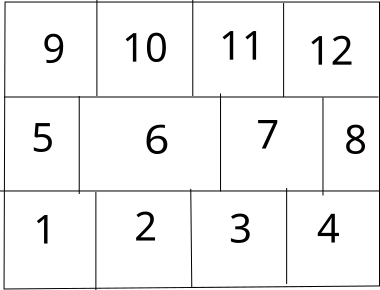
\includegraphics[scale=0.5]{./imagenes/grilla.png}
  \end{figure}

  Definamos la curva \(\gamma_0 (t) := (t, 0)\) que se mueve por el lado
  inferior de \(I \times I\) y cumple que \(F \circ \gamma_0 = \Phi (h)
  \). Análogamente se define una curva \(\gamma_{nm} := (t,1)\) que se
  mueve por el lado superior de \(I \times I\) y que cumple \(F \circ
  \gamma_{nm} = \Phi (g)\). Consideremos a las curvas \(\gamma_k\) como
  aquellas que separen a los rectángulos \(R_1 \dots R_k\) del resto y que
  vayan desde el borde izquierdo al borde derecho. Es claro que
  \[ \forall k,\ F \circ \gamma_k (0) = x_0 = F \circ \gamma_k (1) \]
  es decir, estos son arcos cerrados de \(x_0\). También se ve que
  podemos pasar del arco \(\gamma_k\) al arco \(\gamma_{k+1}\) por la
  homotopía de la linea recta \(\Gamma_k\) contenida en el rectángulo
  \(R_k\), pues el espacio \(I \times I\) es convexo. Por tanto \(F \circ
  \Gamma_k\) es una homotopía entre \(F \circ \gamma_k\) e \(F \circ
  \gamma_{k+1}\).

  Por otro lado, llamemos a las esquinas de los rectángulos \(R_k\)
  vértices. Para cada vértice \(v\) tal que \(F (v) \neq x_0\), sea
  \(g_v\) el arco desde \(x_0\) hasta \(F(v)\). Podemos elegir que
  \(g_v\) tenga su imagen contenida en la intersección de a lo mas tres
  conjuntos \(A_\alpha\) pues por hipótesis, estas intersecciones son
  arco-conexas y contienen a \(x_0\).

  Para todo \(k \in \{1 \dots mn\}\), la curva \(F \circ \gamma_k\)
  tiene una factorizacion por el siguiente procedimiento: Construimos
  una sucesión de arcos (no necesariamente cerrados)
  \[ f_1^{(k)} * f_2^{(k)} * ... * f_l^{(k)} = F \circ \gamma_k \]
  separando a \(F \circ \gamma_k\) en intervalos de manera que queden
  alineados a los vértices de los rectángulos. Esto es un
  procedimiento análogo al utilizado en el teorema
  \ref{thm:vank-especifico}. Entre cada elemento \(f_i^{(k)}\)
  introducimos los caminos \(\bar g _v , g_v\) de ser necesario para
  obligar a que se cumpla
  \[\bar g _v * f_i^{(k)} * g_v \in \pi (A_\alpha, x_0)\]
  Así obteniendo una factorizacion de \([F \circ \gamma_k]\) para todo
  \(k\) tomando las clases de equivalencias (homotópicas) de los
  elementos anteriores y usándolas para formar las cadenas respectivas
  en \(*_\alpha \pi (A_\alpha, x_0)\).

  Esta factorizacion depende de cierto parámetros, puesto que \(\gamma_k\)
  tiene su imagen en las aristas de los rectángulos y potencialmente
  podría darnos varias factorizaciones con elementos en distintos \(\pi
  (A_\alpha)\). Sin embargo, debemos recordar que estas factorizaciones
  seria equivalentes bajo el movimiento dos de factorizaciones descrito
  anteriormente. Mas aun, dado que \(h\) e \(g\) pueden tener
  potencialmente distinta cantidad de elementos en sus cadenas, es
  necesario hacer aparecer elementos extra entre medio mediante el
  segundo movimiento de factorizaciones.

  Por ultimo, notamos que las factorizaciones de \([F \circ \gamma_k]\) e
  \([F \circ \gamma_{k+1}]\) son equivalentes. Esto es debido a la
  homotopía \(F \circ \Gamma_k\), ya que esta solo cambia las curvas en el
  segmento contenido en el rectángulo \(R_k\). Denotaremos a \([a_k,
  a_{k+1}] \subseteq I\) al intervalo tal que
  \[F \circ \gamma_k \, ([a_k , a_{k+1}]) \subseteq R_k\]
  y fijamos un elemento \([f_a^{(k)}]\) de la factorizacion de \([F
  \circ \gamma_k]\) como aquel que le corresponde la seccion del argumento
  \([a_k , a_{k+1}]\). La factorizacion de \([F \circ \gamma_k]\) en
  general correspondera a
  \[ [f_1^{(k)}] [f_2^{(k)}] ... [f_a^{(k)}] ... [f_m^{(k)}] \]
  Por otra parte, la factorizacion de \([F \circ \gamma_{k+1}]\) es
  analoga con su propio elemento \([f_a^{(k+1)}]\) con imagen en
  \(A^{(k)}\) y misma cantidad de elementos.
  \[ [f_1^{(k+1)}] [f_2^{(k+1)}] ... [f_a^{(k+1)}] ... [f_m^{(k+1)}] \]
  Dado que la homotopia \(F \circ \Gamma_k\) solo varia en \(R_k\), se
  tiene que el unico elemento de las imagenes de las cadenas que varian
  son aquellos que pertenece a \(\pi (A^{(k)})\) en el intervalo \([a_k,
  a_{k+1}]\), por lo tanto
  \[ f_a^{(k)} \dot \simeq f_a^{(k+1)} \]
  lo que a su implica la igualdad
  \[ [f_a^{(k)}] = [f_a^{(k+1)}]\]
  por lo que podemos reemplazar los valores en las cadenas. Probando asi
  que son iguales y por tanto equivalentes.

  Luego, dado que \(h\) y \(g\) son factorizaciones de \([F \circ
  \gamma_0]\) e \([f \circ \gamma_{nm}]\) respectivamente y que las
  factorizaciones de \([F \circ \gamma_k]\) son todas equivalentes para
  todo \(k\), se obtiene \(h\) y \(g\) son equivalentes. Por lo tanto
  ambas pertenecen a la misma clase lateral de \(*_\alpha \pi (A_\alpha ,
  x_0)\). Por la arbitrariedad de \([f] \in \pi (X, x_0)\) e \(g,h \in
  *_\alpha \pi (A_\alpha)\), se tiene que el mapeo inducido por \(\Phi\)
  en \(*_\alpha \pi (A_\alpha) / N \to \pi (X,x_0)\) es inyectivo.
\end{proof}
\begin{corolario} \label{cor:vank-trivial}
  Si \(\bigcap_{\alpha \in \tau} A_\alpha \) tiene grupo fundamental
  trivial, entonces
  \[ *_\alpha \pi (A_\alpha , x_0) \simeq \pi (X, x_0) \]
\end{corolario}

Este teorema es largo, pero sus consecuencias son poderosas.
Calcularemos algunos ejemplos que utilicen el teorema de \vank desde
casos sencillos a mas complicados.

\begin{ejemplo}[Espacio ``figura 8'']
El espacio ``figura 8'' en el diagrama es homotopicamente equivalente a
la wedge-sum \(S^1 \vee S^1\).
  \begin{figure}[h]
    \centering 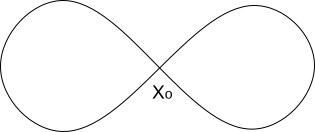
\includegraphics[scale=0.5]{./imagenes/figura8.png}
    \caption*{Espacio figura 8}
  \end{figure}
  Es trivialmente cierto que el conjunto \(\{x_0\}\) es arco-conexo y
  hay inyecciones dos canónicas de \(S^1\) a \(S^1 \vee S^1\). Por tanto
  podemos aplicar el corolario \ref{cor:vank-trivial} para decir el el
  grupo fundamental de \(\left( S^1 \vee S^1 , x_0 \right) \) es \(\pi
  \left( S^1 , x_0 \right) * \pi \left( S^1 , x_0 \right) \).
\end{ejemplo}

El producto libre de grupos \(*_\alpha G_\alpha\) es en la categoría
\(\mathcal{Grp}\) el co-producto categórico. Esto se ve siguiente la
definición \ref{def:coproducto} de co-producto, sean \(X,Y,C\) tres grupos
tales que existan homomorfismo \(\phi_1 : X \to C\) y \(\phi_2 : X \to
C\). Ya se había visto anteriormente como el producto libre \(X * Y\)
admite una extensión (única) de los homomorfismos \(\phi_1, \phi_2\) a
la cual denotaremos \(\Phi : X * Y \to C\), la cual debe cumplir con la
igualdad pedida en \ref{def:coproducto}. Una consecuencia de \vank es
que el functor \(\pi : \mathscr{HoTop}_* \to \mathscr{Grp}\) preserva
co-productos, como fue visto en el ejemplo anterior.

\begin{ejemplo}[Botella de Klein]
  La botella de Klein \(K\) puede presentarse como un cociente en el
  espacio \(I \times I\) representada por el siguiente diagrama.
  \begin{figure}[h]
    \centering 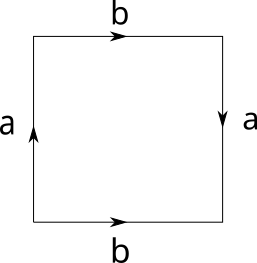
\includegraphics[scale=0.5]{./imagenes/klein.png}
    \caption*{Conjunto \(K\)}
  \end{figure}
  Este espacio puede ser cubierto por los siguientes conjuntos \(U,V\).
  \begin{figure}[h]
    \centering
    
\includegraphics[scale=0.5]{./imagenes/kleinU.png}
    \hspace{3mm}
    
\includegraphics[scale=0.5]{./imagenes/kleinV.png}
    \hspace{3mm}
    
\includegraphics[scale=0.5]{./imagenes/kleinUV.png}
    \caption*{Conjuntos \(U\), \(V\) y \(U \cap V\) respectivamente}
  \end{figure}
  Es claro que \(K = U \cup V\). Elegíamos un punto \(x_0 \in U \cap V\).
  El grupo fundamental \(\pi \left( U , x_0 \right) \) es trivial porque
  este conjunto es convexo y todos los caminos son homotópicas a la
  identidad. El grupo fundamental de \(\pi (V, x_0)\) es isomorfo a
  \(\pi (V, y_0)\) con \(y_0\) el vértice (que identificado es único) de \(I
  \times I\), esto pues el espacio \(V\) es arco-conexo. Estudiando
  \(\pi (V, y_0)\), es claro que \(V\) es homotopicamente equivalente al
  espacio generado por la curvas \(a\) y \(b\) con punto común \(y_0\),
  es decir .
  \[ \pi (V, x_0) \cong \pi (V, y_0) \cong \pi (S^1 \vee S^1, y_0) =
    \mathbb Z * \mathbb Z \]
  tomando a \(a,b\) como generadores.

  Para aplicar \vank debemos estudiar el espacio \(N\). Notese que el
  espacio \(U \cap V\) es homotopicamente equivalente a una curva
  \(\gamma\) contenida en \(U \cap V\) que de una vuelta completa.
  \(\gamma\) es homeomorfa a \(S^1\) y por tanto el
  \[\pi (U \cap V, x_0) \cong \pi (S^1) = \mathbb Z \]
  con \(\gamma\) el generador de este. Debemos estudiar los
  homomorfismos inducidos por la inclusión
  \[ i_{u v} : \pi (U \cap V , x_0) \longrightarrow \pi (U, x_0) \]
  \[ i_{v u} : \pi (U \cap V , x_0) \longrightarrow \pi (V, x_0) \]
  y \(  \pi (U \cap V , x_0) = \langle {[\gamma]} \rangle \). Por
  simple calculo se ve que
  \begin{gather*}
    i_{u v} ([\gamma]) = [\gamma]_{U} = e \in \pi \left( U, x_0 \right)
    \\
    i_{v u} ([\gamma]) = [\gamma]_{V} \in \pi \left( V, x_0 \right)
  \end{gather*}
  con \(e \in \pi \left( U, x_0 \right)\) la identidad de ese grupo y el
  único elemento posible en el recorrido. Véase que \([\gamma]_V\) es
  equivalente homotopicamente a \([a * b * a * b^{-1}]\) por la proyección
  radial desde el centro de \(I \times I\) hacia el borde.
  \begin{figure}[h]
    \centering 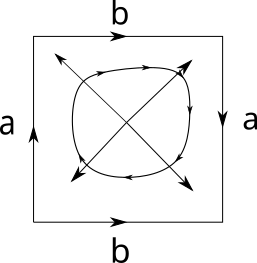
\includegraphics[scale=0.5]{./imagenes/radial.png}
  \end{figure}
  Luego el conjunto \(N\) corresponde al normalizador
  \[ N \{ [a] [b] [a] [b^{-1}]\}\]
  donde este conjunto corresponde simplemente \(\{ [a] [b] [a]
  [b^-1]\}\) con la yuxtaposición como operación, es decir no tiene
  elementos extra de \(\pi (U,x_0) * \pi (V, x_0)\). Luego \vank nos
  dice que se tiene los siguientes isomorfismos
  \[ \pi (K, x_0) \cong \left( \pi (U, x_0) * \pi (V, x_0) \right)
      /_{\{[a] [b] [a] [b^{-1}]\}} = \langle {a , b} \rangle
      /_{\{[a] [b] [a] [b^{-1}]\}}\]
  donde este ultimo puede presentarse como las cadenas generadas por
  \(a,b\) con \(a * b * a * b^{-1} \) reducido o removido por ser la
  identidad, ie
  \[ \langle a,b \rangle /_{abab^{-1} = e} \]
\end{ejemplo}

\subsubsection{Pushout}
Además del producto y el co-producto existen otras estructuras
categóricas que también tienen propiedades universales. Una de interés
en visión de el teorema \vank es la de un pushout. Veremos a
continuación una definición
\begin{definicion}[Pushout]
Sea \(\mathscr{C}\) una categoría. Sean \(X,Y,Z\) objetos en
\(\mathbf{Obj}(\mathscr{C})\) y \(f : Z \to X , g : Z \to Y\) morfismos
en \(\mathscr{C}\). El pushout de \(f,g\) corresponde a una tripleta
\((P, i_1, i_2)\) donde \(P\) es un objeto, \(i_1 : X \to P ,\ i_2 : Y
\to P\) son morfismos de la categoría \(\mathscr{C}\) tales que sean
universales. Esto es, que si existe una tripleta \((Q, j_1, j_2)\) con
\(Q\) un objeto y \(j_1 : X \to Q,\ j_2 : Y \to Q\) entonces existe un
morfismo \(u : P \to Q\) tal que
\[ j_2 = u \circ i_2,\quad j_1 = u \circ i_1 \]
En resumen, el siguiente diagrama conmuta
\begin{figure}[h]
    \centering 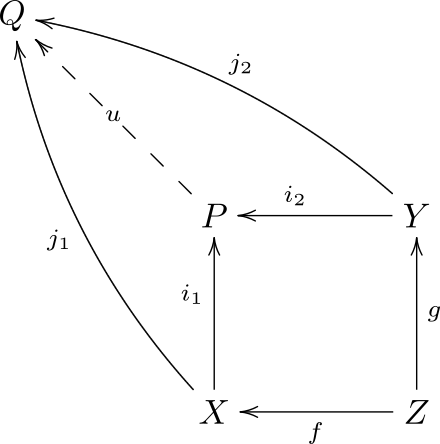
\includegraphics[scale=1]{./imagenes/pushout.png}
\end{figure}
\end{definicion}

El teorema \vank nos dice que hay ciertos tipos de pushout que se
preservan bajo el functor \(\pi : \mathscr{HoTop_*} \mapsto
\mathscr{Grp}\). Notamos que el marco de trabajo de el teorema en la
categoría \(\mathscr{Grp}\) luce como el siguiente diagrama.
\begin{figure}[H]
  \centering 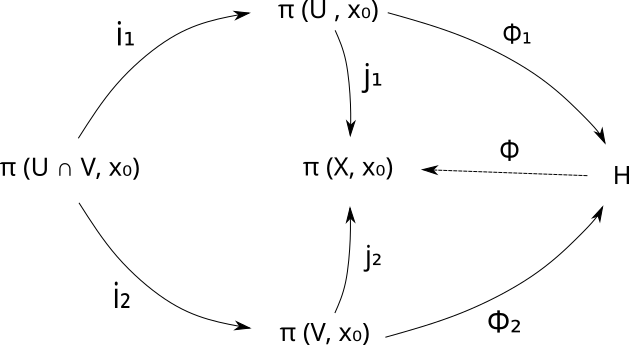
\includegraphics[scale=0.5]{./imagenes/van.png}
\end{figure}
(recordando que estos elementos pierden su notación \(i_*\) por
simplicidad), es decir que el pushout de \(\left( \pi (U \cap V , x_0) ,
i_1 , i_2 \right)\) corresponde a la tripleta \( \left( H , \phi_1 ,
\phi_2 \right)\) con \(H = \pi (U, x_0) * \pi (V , x_0)\) el producto
libre y \(u\) siendo el morfismo \(\Phi\).

Análogamente en \(\mathscr{HoTop}_*\) tenemos los siguiente pushout.
\begin{figure}[h]
  \centering 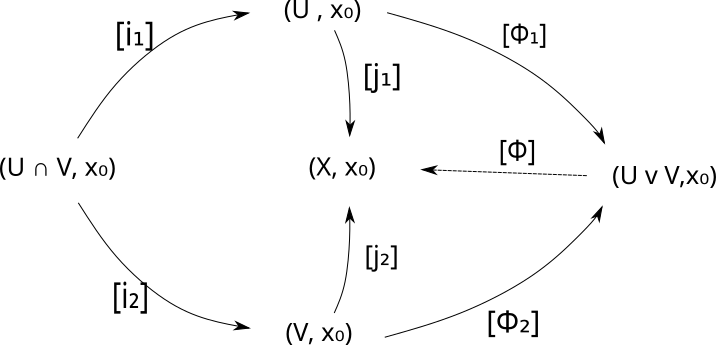
\includegraphics[scale=0.5]{./imagenes/pushoutHotop.png}
\end{figure}
donde \([i_1],[i_2],[\phi_1],[\phi_2]\) son las clases de equivalencias
homotópicas de las inclusiones correspondientes. Esto nos dice que para
la tripleta \(\left( (U \cap V , x_0), [i_1] , [i_2]\right)\) su pushout
corresponde a \(\left( (U \vee V, x_0), [\phi_1], [\phi_2] \right)\) con
\(u = \Phi\).

El teorema de \vank nos dice que si \(\left( U \cap V , x_0 \right)\) es
arco-conexo (hipótesis del teorema) entonces un pushout de \( \left( (U
  \cap V , x_0) , [i_1] , [i_2] \right)\) es preservado bajo el functor
\(\pi\) a un pushout de \(\left( \pi (U \cap V , x_0) , i_{1,*}, i_{2,*}
\right)\). En general no se tiene que se preserven pushouts arbitrarios
bajo este functor. Para resultado mas generales de preservar pushout a
través de este functor se guía a revisar la referencia \cite{brown}.


\begin{thebibliography}{9}

\bibitem{munkres}
  James R. Munkres,
  \emph{Topology},
  Prentice Hall, Upper Saddle River,
  2nd edition,
  2000.

\bibitem{Martin}
  Martin Arkowitz,
  \emph{Introduction to Homotopy Theory},
  universitext, Springer.

\bibitem{Hatcher}
  Allen Hatcher,
  \emph{Algebraic Topology}.

\bibitem{Fraleigh}
  John B. Fraleigh,
  \emph{A first course in Abstract Algebra},
  6th edition.

\bibitem{Bloom}
  Samuel Bloom,
  \emph{fundamental  groups  and  the  Van  Kampen’s theorem}.

\bibitem{brown}
  Ronald Brown and Abdul Razak,
  \emph{A van Kampen theorem for unions of non-connected spaces}.
\end{thebibliography}
\end{document}
